\documentclass{article}
\usepackage{geometry}
\usepackage{fancyhdr}
\usepackage{amsmath , amsthm , amssymb }
\usepackage{graphicx}
\usepackage{hyperref}
\usepackage{wrapfig}
\usepackage{listings}
\usepackage{color}
\usepackage{authordate1-4}
\usepackage{hyperref}

%\usepackage{apacite}

\title{Electoral Engineering through Simulation}
\date{\today}

\begin{document}
\maketitle

% Author and supervisor
\begin{minipage}{0.4\textwidth}
\begin{flushleft} \large
\emph{Author:}\\
Michael \textsc{Fowlie}
\end{flushleft}
\end{minipage}
\begin{minipage}{0.4\textwidth}
\begin{flushright} \large
\emph{Supervisor:} \\
Mark C. \textsc{Wilson}
\end{flushright}
\end{minipage}

\hspace{20cm}

\begin{flushleft}
COMPSCI 380 - Undergraduate Project in Computer Science \\
Semester 2, 2012 \\
University of Auckland
\end{flushleft}

\newpage

\tableofcontents
\newpage

\section{Abstract}
It is claimed in \cite{sweetspot} that the trade-off between expected fairness and stability in election systems is non-linear and that small medium sized District Magnitudes are optimal, based on outcomes of elections in the real world. Does this apply in general or can this effect be explained by other factors? We test the hypothesis that the trade-off is non-linear against artificial societies and across a range of voting systems. We use the Spatial Model, Polya Eggenberger Model and a preference swapping model and the STV, District Proportional and SM rules. Our results show clearly that there is non-linearity in this trade-off however the shape of the curve differs greatly depending on the system we use. We compare these different outcomes under a range of different undesirability functions that value the properties differently. We find that a District Magnitude of $DM=3$, $DM=8$ or $DM=20$ is optimal, depending on how the properties are valued with respect to each other.

\newpage
\section{Introduction}
In relation to election outcomes, there are two properties that we are interested in. These are fairness/proportionality and stability/governability. Under different voting rules (and different parameters for these rules), election outcomes have different tendencies for values of these properties. A high score for each of these properties\footnote{Although as we measure the opposite of these properties, a low score of the opposite is desirable.)} is desirable, however it is well understood that there is a trade-off between the two.

\cite{sweetspot} uses data from 610 elections in 81 countries. It categorised voting rules based on District Magnitude (see Section \ref{sec:DM}). We investigate this trade-off in the context of artificially generated societies and in particular look for non linearity.

We use the STV (see Section \ref{sec:stv}) and DP (see Section \ref{sec:dp}) methods and compare results by varying the District Magnitude (see Section \ref{sec:DM}).

It is claimed that the trade-off between these two properties is non linear \cite{sweetspot}. As District Magnitude increases, fairness usually increases at the expense of stability; however as we demonstrate this is not always the case. Furthermore, in some cases the opposite effect occurs. %TODO Reference

If there is non linearity in the trade-off, it follows that there must be an arguably optimal value of District Magnitude. However there is no clear definition of a desirability function as some people may value one property more than the other.

We compare the results under a number of different undesirability functions which vary the relative contributions of fairness and stability to the result. In each case we calculate the District Magnitudes that optimizes the function in question and thus calculate the District Magnitudes that tend to optimise most of these functions. We find that the optimal case is $DM=3$, $8$ or $20$.

\section{Methodology}
\subsection{Hypothesis}
Our hypothesis $H_1$: There is a non-linear relationship between mean scores for fairness and stability under the different voting systems discussed in Section \ref{sec:votingrules} and various parameters for these voting systems. We use the Gallagher Index (see Section \ref{sec:gallagher}) as a measure of fairness and the ENP Index (see Section \ref{sec:enp}) as a measure of stability, so that our results are comparable with \cite{sweetspot}. We also use one other measure of stability and one other measure of fairness as discussed in Section \ref{sec:enppower} and Section \ref{sec:loosemorehanby} respectively. All permutations of these measures are considered.

\subsection{Procedure}
\subsubsection{Generating Data}
To evaluate the different artificial societies and different voting systems, we consider these in separate runs of the simulator.

In each run of the simulator, we generate a large number of elections for each value of the property that we vary \footnote{This is typically $2000$ although we vary this depending on the computational cost of a simulation.}. This property is usually District Magnitude (see Section \ref{sec:DM}). Each election is generated with a fixed number of seats $S$ and, as the District Magnitude changes, the number of Districts $D$ also changes so that $S=DM \cdot D$. This also forces us to only consider District Magnitudes that are an integer divisor of the number of seats. We chose to consider the case with $S=120$ because it has a large number of divisors and is within an order of magnitude of typical values. This is also the value used in New Zealand. We also considered the case with a larger value $S=(5) \cdot (120)=600$ which is near to the number used in the United Kingdom. We chose $600$ as it is a multiple of $120$ and thus shares all the divisors of $120$.

Each election is generated independently, for example with the Spatial Model we define points for each party and each electorate in the Space of Issues in each election.

\subsubsection{Statistical Analysis}
We fit a regression curve to the measure of fairness and a regression curve to the measure of stability, using DM (see Section \ref{sec:DM}) as the explanatory variable.

see Section \ref{sec:techstats} for technical notes.
\subsection{Tools}
The simulator itself consists of a library written in the Visual C\# \textregistered \footnote{Visual C\# and Visual Studio are either registered trademarks or trademarks of Microsoft Corporation in the United States and/or other countries.} $ $ 5.0 programming language along with scripting code written in the Visual C\# and Visual F\# 2.0 programming languages (F\# is a variant of the ML functional programming language). Code was written using the Visual Studio \textregistered $ $ 2010 and Visual Studio 2012 IDEs and the RGui and Notepad++ editors. Simulations are performed on \href{http://aws.amazon.com/ec2}{Amazon EC2\texttrademark\footnote{Amazon Web Services, the "Powered by Amazon Web Services" logo, EC2 are trademarks of Amazon.com, Inc. or its affiliates in the United States and/or other countries.}} c1.xlarge instances with Intel \textregistered \footnote{Intel, Xeon and Pentium are trademarks of Intel Corporation in the U.S. and/or other countries.} $ $ Xeon \textregistered $ $ E5410 processors and a workstation with an Intel Pentium \textregistered $ $ G620 processor.

Data from \cite{nzes08} was imported and processed with scripts using SAS \textregistered \footnote{SAS and all other SAS Institute Inc. product or service names are registered trademarks or trademarks of SAS Institute Inc. in the USA and other countries. \textregistered $ $ indicates USA registration. } software and Visual C\#.

The resulting dataset is then analysed using R 2.15.1.

\section{Measures}
We actually measure the \emph{opposite} of the desirable properties, that is, we measure unfairness and instability.

Unfairness and Instability are measured in a variety of ways as described below.

Note that in our plots we normalize measures so the minimum value for each property is optimal. For the measures \ref{sec:enp} and \ref{sec:enppower} this involves subtracting $1$ from the values so that $0$ is optimal. For the measure \ref{sec:entropysspi} we multiply the values by $-1$ so that lower plotted values are better. The Gallagher Index and Loosemorehanby Index are already optimal with values at $0$.

\newpage
\subsection{Measures of Unfairness}
We define $\delta_i$ such that
$\delta_i = v_i - s_i$

where $v_i$ is the proportion of votes of party $i$ and

$s_i$ is the proportion of seats of party $i$.

\label{sec:loosemorehanby}
We use the Loosemorehanby Index $D=\frac{1}{2} \sum_{i=1}^m \arrowvert \delta_i \arrowvert$

\label{sec:gallagher}
and the Gallagher Index $D = \sqrt{\frac{1}{2} \sum_{i=1}^m \delta_i^2}$. \cite{gallagher}
\subsection{Measures of Instability}
\subsubsection{Effective Number of Parties}
\paragraph{}
\label{sec:enp}
As a measure of ungovernability, we use the Effective Number of Parties. $ENP=\frac{1}{\sum_{i=1}^m p_i^2}$ \cite{enp} where $p_i$ is the proportion of seats that party $i$ has and $m$ is the number of parties.
\subsubsection{ENP using Shapley Shubik Power Index}\label{sec:enppower}
\paragraph{}
As for the purposes of governability, only power is relevant (as opposed to the proportion of seats), it seems reasonable to modify the ENP formula to use political power instead of the proportion of seats, by party. $ENP=\frac{1}{\sum_{i=1}^m SSPI_i^2}$

$SSPI_i$ denotes the Shapley Shubik Power of party $i$.

We consider an arbitrary order over all parties. We consider all parties ranked before party $i$ to be part of one coalition and all parties ranked after party $i$ to be part of another coalition. We repeat the analysis for every possible permutation over all parties and every possible value of $i$ in the case of each permutation.

Party $i$ is not considered to be part of either coalition. Party $i$ is pivotal if and only if party $i$ joining one of the two possible coalitions would cause either to become the majority depending on which it joins\footnote{i.e. the coalition has more than $0.5$ of the total vote share.}. We define $pivotal_i$ to be the number of times party $i$ is pivotal over all possible orders.

$SSPI_i = \frac{pivotal_i}{\sum pivotal}$ \cite{shapleyshubik}

i.e. $SSPI_i$ denotes the proportion of orders in which party $i$ is pivotal.

For example a parliament with a party having $0.51$ of the seats has the same amount of governability as one with a party with $0.99$ of the seats. In both of these cases the party in question has all of the power as defined by the Shapley Shubik power index, however the ENP formula distinguishes between these two cases.

\paragraph{}
This measure has, in some cases, the interesting effect of measuring an increase of stability when reducing the threshold under MMP. Consider the following election (See Figure \ref{tab:shapleyshubikpower}) where $v_i$ denotes the number of votes of party $i$, $p_i$ denotes the Shapley Shubik power of party $i$ with a 10\% threshold, and $q_i$ denotes the Shapley Shubik power of party $i$ with a zero threshold. Note that a \emph{lower}  value for ENP is considered more stable.

\begin{figure}[h!b]
\begin{tabular}{l l l }
\hline
Votes & $p_i$ & $q_i$ \\ \hline
47 & 0.3333 & 0.6667 \\
26 & 0.3333 & 0.1667  \\
26 & 0.3333 & 0.1667  \\
01 & 0.0000 & 0.0000 \\ \hline
$\sum_{i=1}^m SSPI_i^2$ & 0.3333 & 0.5000 \\
$\frac{1}{\sum_{i=1}^m SSPI_i^2}$ & 3 & 2 \\
\hline
\end{tabular}

\caption{Under some elections, increasing the number of parties increases stability when measuring as described in section \ref{sec:enppower}.}
\label{tab:shapleyshubikpower}
\end{figure}

\subsubsection{Entropy of Shapley Shubik Power}
\label{sec:entropysspi}
\paragraph{}
We also consider the entropy of the Shapley Shubik index. $\sum_{i=1}^m SSPI_i \cdot \ln(SSPI_i); SSPI_i \neq 0$
\section{Artificial Societies}
In each society we define $m$ parties and $M=m!$ preference orders, where a preference order is an order over all parties.
We define $n$ as the total number of voters in a given district.

\subsection{Polya Eggenberger (Urn) Model}
In each district we sample $n$ preference orders, each representing a single voter, from the Polya Eggenberger distribution with parameter $a$ where $a$ represents the homogeneity of preferences in a given district. We assume independence of districts and there is no bias in favour of any particular party, as the number of districts approaches $\infty$ the distribution of votes to parties will approximate a uniform distribution - thus this model is not very realistic.
% TODO: Note about not being interesting for the purposes of Apportionment Methods.

%Explain the Urn process
\subsubsection{Urn Process}
The Polya Eggenberger distribution can be understood via intuition from the urn process. The urn contains multiple balls, each of a different colour (where a colour represents preference order). To sample using the urn process we select a ball from the urn uniformly at random, record the colour, and place the ball and $a$ copies of the ball into the urn. We define the weight of a preference order (colour of ball) to be equivalent to the number of balls in the urn, and the weight of the urn to be equal to the total weight of all colours of balls in the urn, however, it is important to note that $a$ (and thus weight) need not be an integer.
\subsubsection{Parameter selection}
We use both the case with a constant $a$ for all districts, and the case for a random $a$, where we first define $b=U(0,1)$ and then let $a=b/(1-b)$.

\subsubsection{Sampling}
A naive approach to sampling a value $x$ from the Polya Eggenberger distribution would be to store the weights of each preference order in a vector $w$ then select a value uniformly at random $y=U(0,\sum_{i=1}^M w_i)$ then select the minimum value of $x$ such that $\sum_{i=1}^{x}(w_i) \geq y; x \leq M$. We would then adjust the weight for the selected preference order $w_x$ by adding $a$.

This has time complexity of $O(M)$ per sample, or $O(n \cdot M)$ to sample a single district, and space complexity $O(M)$. Note that $M=m!$ can be quite large. We use a more efficient method to sample, by replacing $x$ with a compressed data structure (see Section \ref{sec:efficientsampling}) with worst case space complexity $O(min(n \cdot \ln (M),M))$ and worst case time complexity $O(n \cdot \ln M)$ (per district) which is less than $O(n \cdot m \ln m)$
%TODO Describe turning integers to preferences orders and back again.
\subsection{Spatial Model}
\label{sec:spatialmodel}
%Describe parameters to our model.
%Describe parameter z.
Our model has a parameter z which is a vector representing the standard deviation in each dimension in the space of issues where $z_j \geq z_{j+1}$

%Argue why |z|=m
%TODO: Prove this?
% As our model is unaffected by adding dimensions with zero variance, that is values of $j$ such that $z_j=0$, it would still be possible to fit our model with an overestimate of $|z|$, and for $|z|>m$, there exists an equivalent model with $|z|=m$, thus for the sake of convenience we define $|z|=m$.

%Describe parameter d.
We have a parameter $d$ which represents the standard deviation of population means of districts as a portion of the standard deviation of voters.

%Space of issues
We define a dimensional space $|z|$ called the space of issues. Each voter and each party are represented by a point in this space. Voters prefer parties with a lower distance between a voter's point and a given party's point.
In each party $i$ we select $p_{i,j}=N(0,z_j)$ where $p_i$ represents the point in the space of issues of party $i$.
We also consider the case in which two of the parties represent the traditional major left and right parties\footnote{In this case both the left and right parties have points almost at the origin. e.g. $(+0.0001,0)$ and $(-0.0001,0)$.}.
Population means for voters in a district $k$ is selected $\mu_{k,j}=N(0,z_j\cdot d)$ We assume districts are independent.
In each district $k$, a voter $n$ is selected $v_{n,j}=N(\mu_{k,j},z_j)$
\subsubsection*{Parameter selection}
An obvious class of parameter values to select are all non-zero variances set to be equal, with $1$, $2$ or $3$ non-zero dimensions. In particular two dimensions is interesting as the dimensions can refer to economic liberty and social liberty. %TODO: Rephrase this

We fit parameters to this model, obtained from real world data, via the method discussed in Section \ref{fittingrealworldENI}.

\subsection{Preference Swapping Model}
\label{sec:prefswapping}
\paragraph{}
The Preference Swapping Model extends upon the model used in the 2011 referendum simulator \cite{nzreferendumsim}. It takes a set of real world elections as a parameter and creates a cluster of similar elections around each real world election. The model works by redistributing real election results, evolving an input election by inferring the preference orders for each vote and switching preferences by some transformation function.

The transformation function for preference orders works by switching the order of the preferences with some probability. The probability of switching between 1st place and 2nd place may be different from switching between 1st place and 3rd place, for example. As we are only concerned with 1st place preferences, we do not consider the case where another pair of preferences also switches. We also use the case where we apply the output of our model as the input to another stage in our model (e.g. so that we model 2 or more steps into the future). Each stage is calculated in the same way; with the exception that we infer preference orders only from the first preferences in the first step.

%TODO How we reorder preferences. (i.e switching 1 and 3, returns 3 1 2 4 or 3 2 1 4?)

\paragraph{}
We define $s_i$ to be the probability that a voter switches the 1st and $i$th preference, where $s_i$ is selected uniformly at random between $0$ and $\max(s_i)$ where $\max(s_i)$ is a parameter to our model.

It doesn't make much sense for $s_i < s_{i+1}$ however, even with $max(s_i) > max(s_{i+1})$ (as we would expect), our model can generate values of $s_i$ and $s_{i+1}$ such that $s_i < s_{i+1}$. We consider both the case where we apply no additional restrictions on the model and the case where $s_i \geq s_{i+1}$

\subsubsection{Redistricting}
%TODO
It was not required to generate $D_{new}$ \footnote{Recall that $D$ represents the number of districts.} new districts that each were strictly a combination of the original districts and that each original district was used once. It was only required that after redistricting we would get similar results than if we had done this.

Redistricting is done by the following algorithm:

\begin{itemize}
\item Calculate the principal components of districts \footnote{We calculate the principal components of a dataset with rows representing districts and columns representing parties. A cell represents the proportion of votes in a given district that were for a given party.} and the distribution of the deviations for each principal component\footnote{Assuming the deviations are normally distributed.}.

\item Generate modified distribution for each principal component by selecting a new standard deviation for each $SD_{new} = SD_{old} \cdot \sqrt{\frac{D_{new}}{D_{old}}}$ \footnote{This reduces or increases the variance of the deviations in accordance with the Central Limit Theorem. With a smaller number of districts, one would expect each district to have a closer distribution of votes to the mean than the case with a larger number of districts.}.

\item In the case of each new district, we sample from the modified distributions of principal component deviations and back-transform these deviations into district information. In the case that the generated information is invalid \footnote{We consider a generated district to be invalid if any party receives a negative number of votes.} we try this step again, otherwise we keep the information and continue.
\end{itemize}

The resulting districts will have total vote proportions by party that is approximately equal to the total votes proportions by party of the original data.

\subsubsection*{Parameter selection}

We use the 2011 election in New Zealand as a start point and infer preference orders and the probability of switching preference orders from the NZES 2008 \cite{nzes08}.

We infer preference orders from the survey by assuming that the first preference of a voter is the party that the voter actually voted for and that the remaining parties are ordered in descending order based on the scores that voters were asked to rate parties by.

We found that $18\%$ of voters switched between their first and second preference, and $12\%$ switched between their first and third preferences. We do not consider switching between preferences lower than 3rd as our preference data is not reliable enough. We select $\max {s_2}=0.18$ and $\max {s_3}=0.12$.

%TODO: Make this better. Explain the case where a voter gives the same score to multiple parties.
In the case where voters gave the same score to more than one party, we consider all possible orders of parties with the same score with the weight for each score reduced accordingly.

%Explain transformation to matrix for transforming first preferences (from actual elections) to full preference data for an election.
We normalise the weights for all preference orders where voters voted for a given party to $1$, then treat the normalised weights as a probability that a voter for a given party has a particular preference order.

We assume that given a voter voted for a particular party, the probability it has a particular preference order is independent of its district and from election to election.

%Explain how we obtain s_i.

We select $s_i$ to be the proportion of voters whose vote in 2005 (the previous election) was equal to their $i$th current preference.

\section{Apportionment Methods}
\label{sec:apportionment}

Apportionment methods ensure that when rounding to integers, in this case vote shares to seat shares, we can minimise error (for some definition of error), while rounding to a constant total.

We let $p_i$ be the proportion of votes that party $i$ receives and we define apportionment functions that transform $p$ to $s$ where $s_i$ is the seat share of party $i$.

The true number of seats a party $i$ deserves is $t_i = |s| \cdot p_i$, however $t_i$ may not be an integer.

In the case of each method we define $l_i = floor(t_i)$ and $s_i = l_i + k_i$ where $k_i$ is either $0$ (we round down) or $1$ (we round up).

It follows that $\sum{s}=\sum{l}+\sum{k}$ and thus $\sum{k}=\sum{s}-\sum{l}$

The methods differ on how $k$ is defined.

To resolve the case of ties, we add a small vector of additional random votes totalling less than $1$ real vote.
\subsection{St Lague Method}
We do not calculate $k$ directly. In this method we iteratively allocate $|s|$ seats.

In each iteration we allocate the next seat to the party with the highest quotient where $quot_i=\frac{v_i}{2s_i+1}$
\subsection{D'Hondt/Jefferson Method}
The D'Hondt and Jefferson methods are mathematically equivalent in that they both return the same results, though they are calculated differently.

We generate an $m \cdot |s|$ matrix \footnote{Recall that $m$ is the number of parties.}. Values in the cells are set such that $(i,j)=\frac{v_i}{j}$

We then select a cut-off threshold such that there are only $|s|$ values in the matrix that are above the cut-off.

Each party $i$ is allocated as many seats as there are values of $j$ such that the value in cell $(i,j)$ is greater than the threshold.
\subsection{Hill Method}

We iteratively allocate each seat. In each iteration we allocate the next seat to the party with the highest quota, where $quot_i=\frac{v_i}{\sqrt{floor(s_i)^2+(floor(s_i)+1)^2}}$
\subsection{Hamilton Method}
We already know $\sum k$, we allocate $k_i=1$ to the values of $i$ in descending order of $t_i-l_i$ for $\sum k$ values of $i$.

\section{Fitting real world data to the Spatial Model}
\label{fittingrealworldENI}
It is of interest to calculate parameters for the Spatial Model (see Section \ref{sec:spatialmodel}) that are reasonably like the real world. To do so we attempt to fit real world data to the spatial model.

We assume that there is a relationship between the parameter $z$ and the proportion of variance explained by each principal component of the results per party by district. 

%From Section \ref{sec:numberofissues}, we assume that we need only to fit an $ENI$ value. %Describe our hypothesis
%We hypothesise that the same formula used for calculating ENP and ENI applied to the portions of variance explained by each principal component of the number of first preferences of a %each party by district will have a relationship with $ENI$. %TODO Evidence of this

%Efforts to validate the hypothesis
We attempt to validate this hypothesis by simulating a large number of elections under our model, several for each of many different values of $z$ and compare it to the values obtained when applying the formula to the variance from principal components of the election results. See Figure \ref{fig:spatial_var_pca}. %TODO Update figure.

%Evidence in support of this idea.
\begin{figure}[]
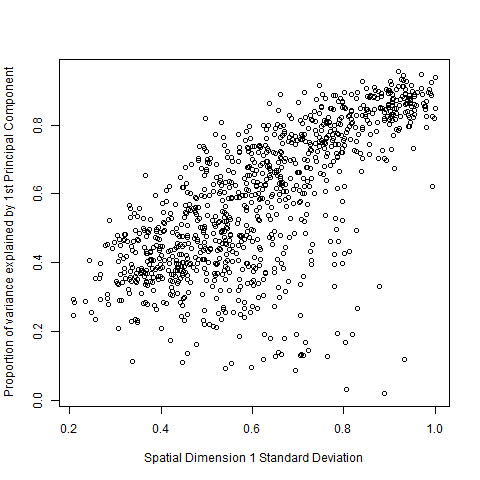
\includegraphics[scale=0.75]{images/spatialvar1_pcavar1.png}
\caption{Values of $z_0$ vs proportion of variance explained by the first principal component}
\label{fig:spatial_var_pca}
\end{figure}

We fitted a regression line and found extremely strong evidence $p-value < 2 \times 10^-16$ against $H_0$ that there was no relationship between the two variables. The fit had high error $R^2=0.49$ but this error can be mitigated by taking a large number of samples from artificial societies for a given $z$ value and comparing distances to a reasonably large set of real world elections.

%How this allows us to find values for z.

We select $z$ as to minimise the error of the model in describing a set of real world elections. We recursively select smaller and smaller ranges that we predict contain the target value of $z$ to minimise the error as follows:

%TODO: Explain why we can using y to explain most of the variation %

We define $y = \sum_i {z_i}^2$ 

\begin{itemize}
\item 1. Generate several values uniformly at random within the range of $y$ values that we believe the target $y$ to be in.
\item 2. Find a value of $z$ with $y$ close to our target and update the values of $y$ with the actual values from our values of $z$
\item 3. For every value of $z$ we simulate a number of elections and compute the mean error.
\item 4. Select all the results (by $y$ value) that have the minimum mean absolute error, and discard the rest.
\item 5. Calculate the underlying distribution of $y$ values that we retained in step 4. (assuming a Normal distribution)
\item 6. Calculate new upper and lower bounds for the target $y$ value. If these bounds are within our target error margin we select mean, otherwise we loop with these new bounds.
\item 7. Select a $z$ value from a number of generated candidates with the target $y$ that minimises the error.
\end{itemize}

We found that this method can, with reasonable accuracy, calculate $z$ values from election outcomes generated from the spatial model, however it had higher error from real world election outcomes and the results varied each time we ran the algorithm. We found that the values of $z$ the algorithm found from real world data was not unlike the parameters we were using in the simulation.

%TODO Alternative ways we tried? i.e. Newton Raphson with our modification?

%TODO Define distance.

%TODO: Actual results
%TODO \paragraph{Parameter d}

%TODO
%\section{Redistricting real world data}
%For the purposes of the simulator, in particular with the Preference Swapping Model, it was of interest to simulate many artificial societies that are similar with regard to certain %properties to the real world. 

%Redistricting is known to be NP complete. %Citation?

%However in the simulation, it was not required when redistricting for our new districts to strictly be a combination of the old districts - only that the resulting districts have %equivalent properties to this.

\section{District Magnitude}
\label{sec:DM}
District Magnitude represents the number of seats in a particular district. \cite{sweetspot} uses the median district magnitude to group collections of voting rules and their parameters for analysis. In some systems (e.g. SM, see Section \ref{sec:SM}) the district magnitude varies from district to district. Using the median would group SM in the same category as FPP which is undesirable. We resolve this problem by analysing voting systems independently instead of grouping the data together. We use the median in all cases except the case of SM, in which case we use the district magnitude of the largest district.

\section{Voting Rules}
\label{sec:votingrules}
\subsection{Single Transferable Vote}
\label{sec:stv}
In this system we take into account the complete preference orders of voters. We define a number of equal sized districts and define a quota, such that $quota=(\frac{n}{DM+1})+1$. (where $n$ is the number of voters in a given district)

All parties need to obtain $quota$ votes to obtain a seat. The process of allocating votes to parties, in each district, works as follows:

\begin{itemize}
\item 1. Assign a weight $w$ of $1.0$ to all votes. The system can be optimised by combining identical votes and using the sum of their weight.
\item 2. Calculate the sum of weights $\omega = \sum_i{w_i}; p_{i,1}=j$, by party $j$, for all votes. Select the party to assign the weight by the highest non-excluded and party in a voter's preference order\footnote{$p_{i,k}$ denotes the $k$th non excluded preference of voter $i$.}.
\item 3. Each party that obtains a weight greater than or equal to the quota is elected. We reduce the weights of all votes that have the highest non-excluded preference equal to a given elected party by multiplying each by $m = \frac{\omega - quota}{\omega}$, thus there is $quota$ weight removed.
\item 4. If no party was elected in Step 3, we exclude the party that obtained the least weight in Step 2.
\item 5. We loop back to Step 2. until enough parties are elected.
\end{itemize}

\subsection{Proportional Systems}
We use the following two voting systems which are special cases of a more general system which is proportional in each district. At one extreme of both of these systems is FPP (First Past the Post), and the other extreme, pure proportional. In each district under these systems, we apply some apportionment method (see Section \ref{sec:apportionment}) to select the number of seats by party, and aggregate the results. These systems take into account only first preference votes.
\subsubsection{District Proportional}
\label{sec:dp}
In this special case, we define multiple districts of equal size. Each voter votes under only one district.
\subsubsection{Supplementary Member}
\label{sec:SM}
In this special case, we define a number of districts of size $1$ and a single large district of some larger size. Voters are assumed to each vote in one of the smaller districts and to all also vote in the larger district. We assume voters vote the same way for both the small district and the large district.

\section{Efficiently Sampling from a Discrete Probability Distribution}
\label{sec:efficientsampling}
We define $w_i$ to be the weight of element $i$ in the probability distribution, where $Pr(X=i)=\frac{w_i}{\sum w}$
We take advantage of the fact that most elements in the probability distribution have a weight of 1. However this structure does not actually store $w$ directly.

The structure is similar to a binary search tree, however instead of containing elements it contains \emph{ranges} where leaf nodes (i.e. nodes with a range length of $1$) represent the elements of $w$. Every element in the tree contains a precomputed parameter representing the weight of the element, where we define the weight of a non-leaf node (that is, a node that doesn't represent a single element) to be the sum of the weights of its left and right child. Much of the tree is not ever written to, or read from, and so we can lazily load nodes on demand. This lazy loading saves us a significant amount of space for a large $|w|$.

\paragraph{}
When sampling from the distribution, we select a value $y$ uniformly at random $y=U(0,\sum w)$ and call a recursive search function on the root node, as defined by the below pseudo-code:

\begin{lstlisting}[language=C++]
Node RecursiveSearch(Node n, double y)
{
	if (n.length == 1)
		return n;
	
	double skipAmount = 0.0;
	
	if (getLeftChild(n) != null)
	{
		if (getLeftChild(n).weight>=y)
		{
			return RecursiveSearch(getLeftChild(), y);
		}
		else
		{
			skipAmount = getLeftChild(n).weight;
		}
	}
	
	return RecursiveSearch(getRightChild(n), y - skipAmount);
}
\end{lstlisting}

Once the node in question is found, we return the sampled value from the distribution and update the weight of the node by the requested amount. When increasing the weight of an element, we need to increase the weight of the parent node \footnote{By updating the parent's weight, the weight of the parent's parent must also be updated, etc.} which takes, in the worst case, $\ln |w|$ time.

\section{Undesirability}
\label{sec:undesirability}
%TODO

We define an undesirability function to be a function of both unfairness and instability which returns a real number which is optimal when minimised. Different functions have different levels of sensitivity to each of these properties. For the purposes of this analysis we consider only linear functions so as to minimise the number of arbitrary parameters we use.

It seems unreasonable to define a linear undesirability function that has a coefficient for either unfairness or instability that is less than zero \footnote{In the case of a linear undesirability function with coefficients less than zero, we would consider a less unfair or less unstable result to be more undesirable, that is, a more fair or more stable result to be undesirable.}, thus only functions with coefficients equal to or greater than zero are considered. We transform unfairness and instability by first dividing each by its corresponding standard deviation across our entire dataset \footnote{This is in an attempt to neutralise any bias in our choice of random undesirability functions.}. We do not need to bother about constant errors \footnote{Subtracting a constant from either as we only ever consider minimising undesirability across the same undesirability function and a constant added to the function would clearly be constant across all values from that function. Likewise, multiplying by a positive constant would have the same effect across all values of the function and thus we only need to consider one undesirability function of any set of undesirability functions that can be transformed by a linear function from one to the other.}. We construct an undesirability function by first creating a line $L_1$ from the optimal point \footnote{The origin $(0,0)$ after transforming the properties as described above.} to a point along the line segment $L_2$ $(1,0)$ to $(0,1)$. We consider $L_2$ to be an axis that we measure the plotted transformed point of unfairness and instability against.

We subdivide $L_2$ into a large number of equal length parts and consider the undesirability functions that are defined when $L_1$ intersects $L_2$ at each different boundary of these different subsections of $L_2$.

As we are interested only in minimising undesirability across multiple values of District Magnitude, we compare only the undesirability of average points for each District Magnitude.

In reality, only undesirability functions that intersect close to the midpoint of $L_2$ are worth considering. Extreme values correspond to only caring about one property.

\section{Results}
\subsection{Simulation Results}

The outcomes from a series of simulation runs are plotted below. For each run, four plots are provided. The bottom left corner of each plot is optimal. Points in the top left plot represent individual simulations in a given run. Points in the top right plot represent means predicted, in accordance with our regression model, for a given District Magnitude. The bottom left plot may be slightly misleading as points plotted here are not necessarily near results from actual simulations. Each point represents a single District Magnitude and the position along each axis refers to the 95th percentile value for simulations using this District Magnitude. The purpose of this plot is to demonstrate the worst expected values for each of the two properties plotted. Points in the bottom right plot represent means, from actual results, per District Magnitude.

There is a cluster of results in the bottom centre-right of Figure \ref{fig:stv_spatial2_sspi}. This represents the case when a single party has all the Shapley Shubik Power.

Supplementary Member (See Figure \ref{fig:sm_spatial2}) has a much different curve than for the other rules \footnote{Recall that District Magnitude for Supplementary Member is defined differently. By the definition we use for the other systems, SM would have $DM=1$ in all cases}.

The results in Figure \ref{fig:stv_nzprefswap} are generated using the Preference Swapping Model (Section \ref{sec:prefswapping}) using spatial information obtained from \cite{nzresults2011} and preference information obtained from \cite{nzes08}.

Unless otherwise stated, results are calculated with $120$ districts and $8$ parties and results calculated with the spatial model include major left and right parties.

\begin{figure}[]
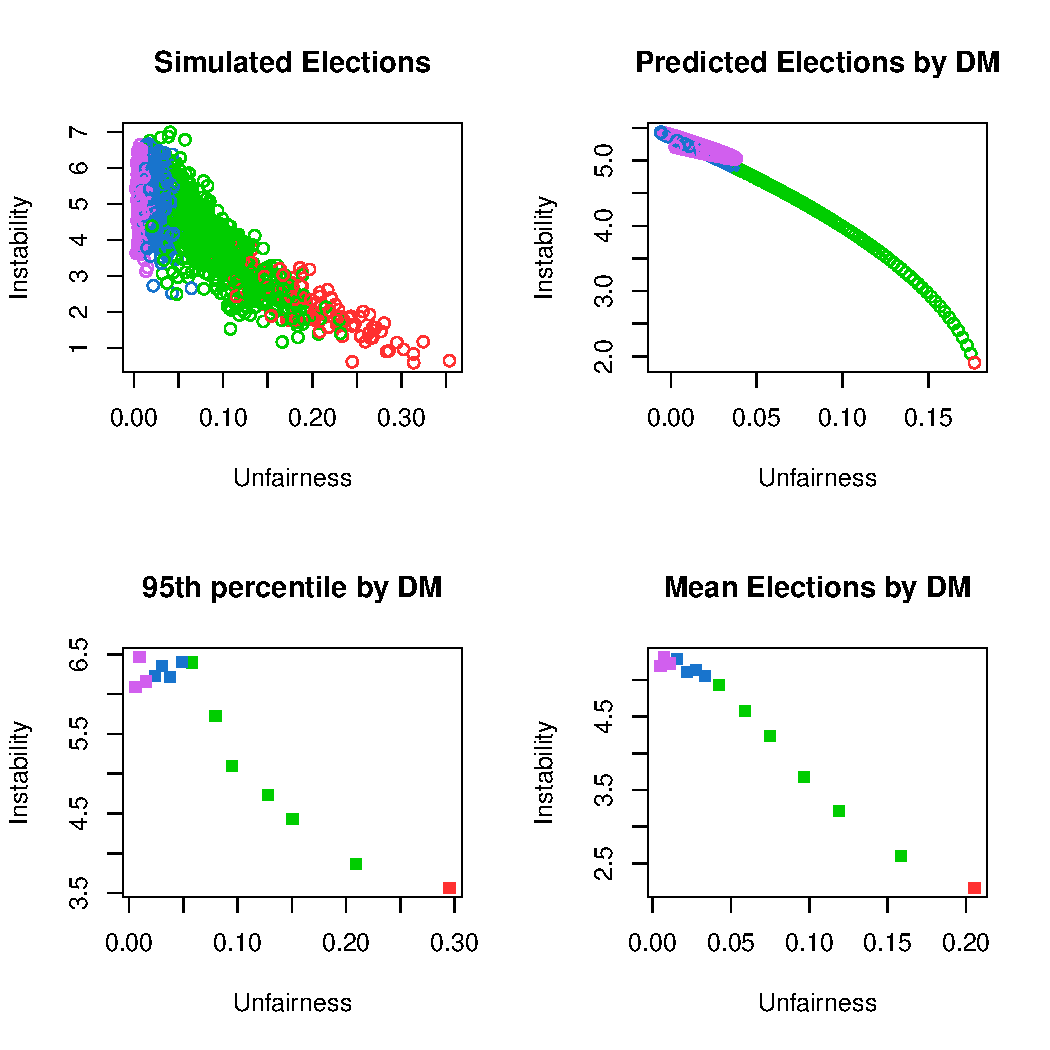
\includegraphics[scale=1.00]{images/pd_spatial2_gallagher_enp.pdf}
\caption{Results from simulated elections with the \emph{Spatial Model} with \emph{$2$ dimensions} and the \emph{District Proportional} rule. Plotted using the \emph{Gallagher} Index vs. \emph{ENP}. DM=1 (Red) DM=2-9 (Green) DM=10-29 (Blue) DM$>$30 (Purple)}
\label{fig:pd_spatial2}
\end{figure}

\begin{figure}[]
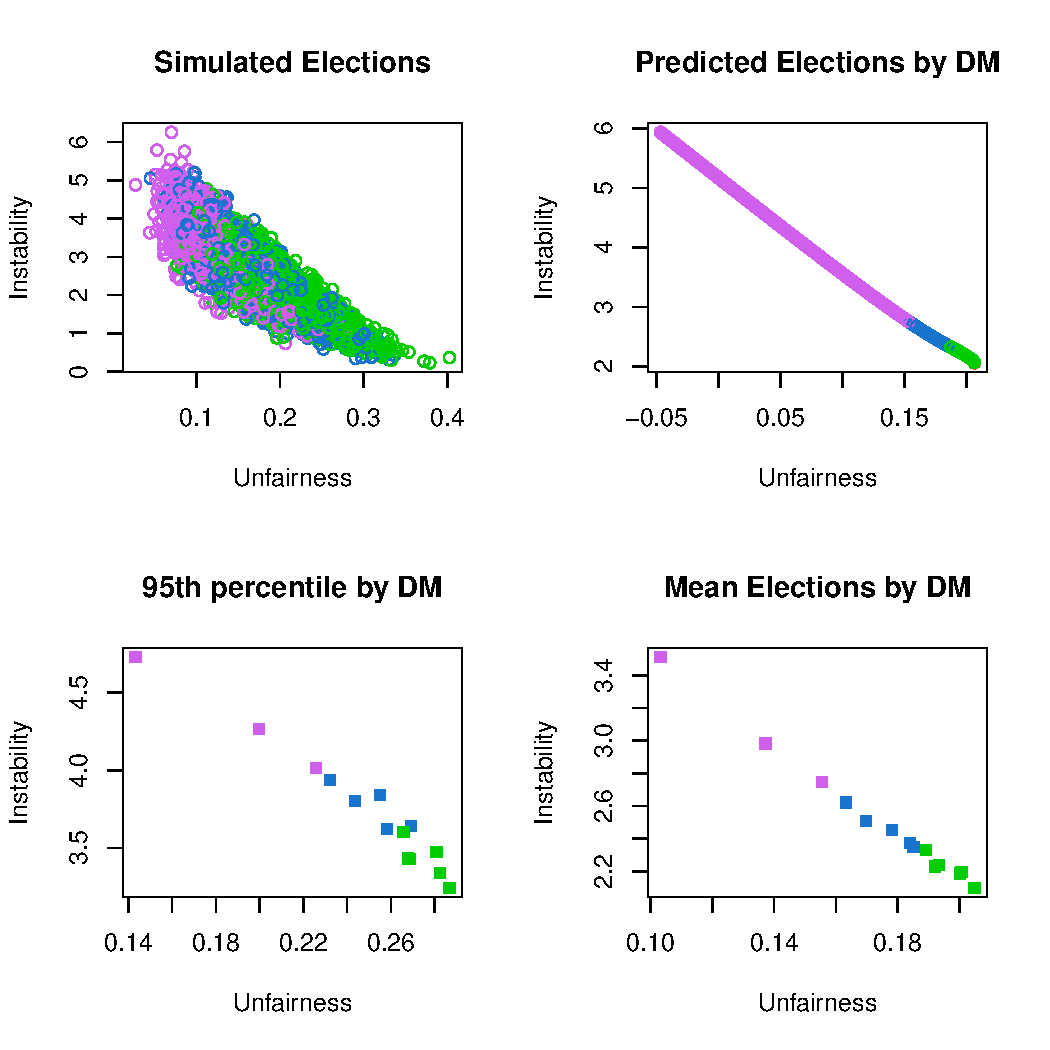
\includegraphics[scale=1.00]{images/sm_spatial2_gallagher_enp.pdf}
\caption{Results from simulated elections with the \emph{Spatial Model} with \emph{$2$ dimensions} and the \emph{Supplementary Member} rule. Plotted using the \emph{Gallagher} Index vs. \emph{ENP}. DM=1 (Red) DM=2-9 (Green) DM=10-29 (Blue) DM$>$30 (Purple)}
\label{fig:sm_spatial2}
\end{figure}

\begin{figure}[]
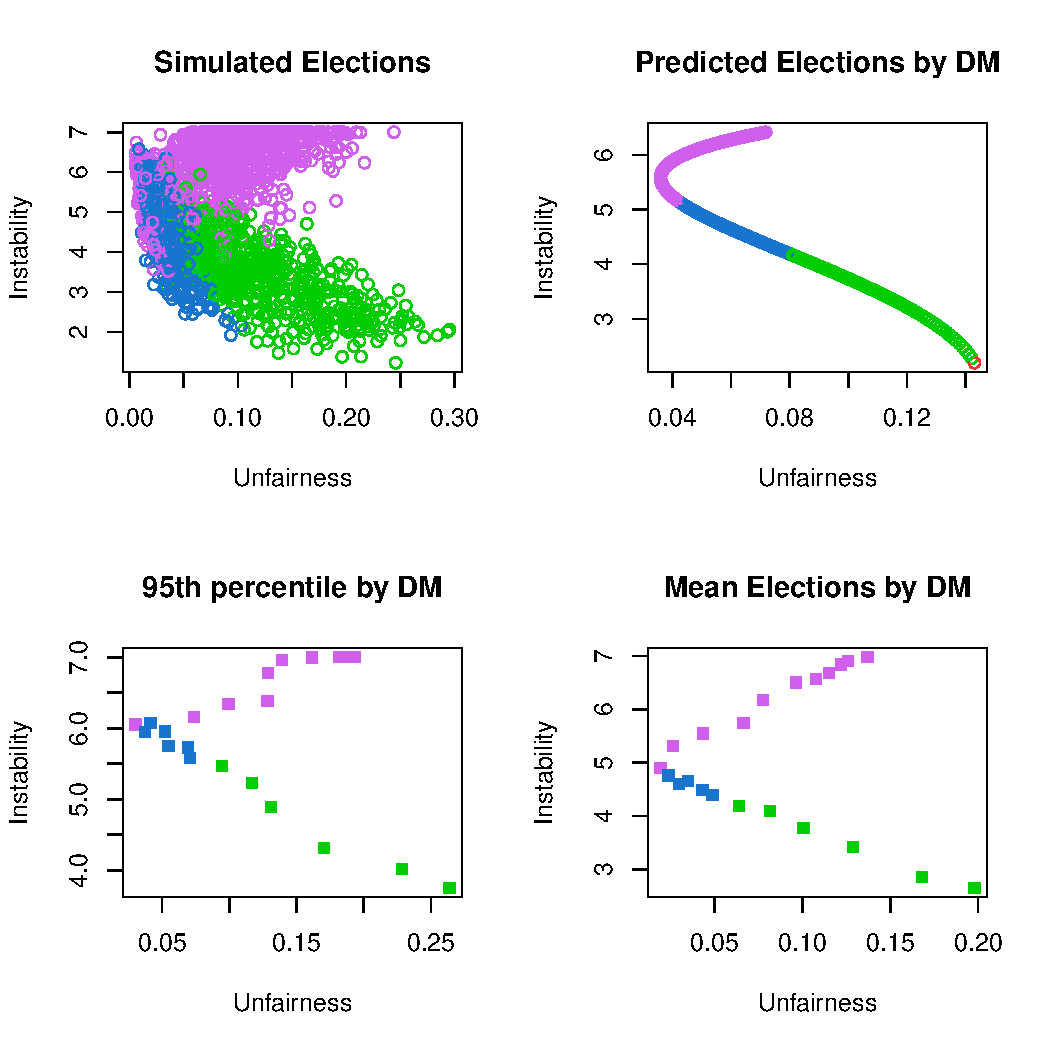
\includegraphics[scale=1.00]{images/spatial2large_gallagher_enp.pdf}
\caption{Results from simulated elections with the \emph{Spatial Model} with \emph{$2$ dimensions} and the \emph{STV} rule. Plotted using the \emph{Gallagher} Index vs. \emph{ENP}. DM=1 (Red) DM=2-9 (Green) DM=10-29 (Blue) DM$>$30 (Purple)}
\label{fig:stv_spatial2}
\end{figure}

\begin{figure}[]
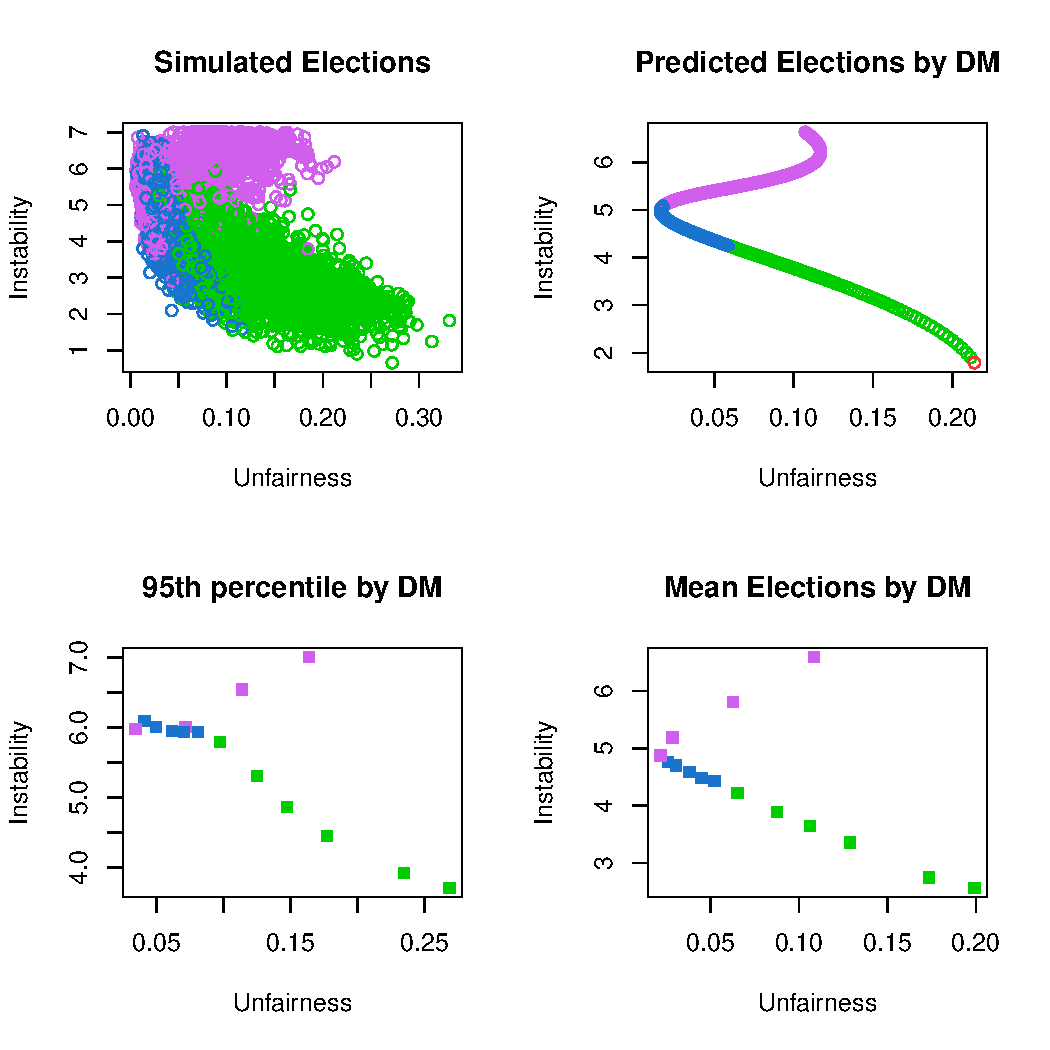
\includegraphics[scale=1.00]{images/stv_spatial2_gallagher_enp.pdf}
\caption{Results from simulated elections with the \emph{Spatial Model} with \emph{$2$ dimensions} and the \emph{STV} rule with \emph{600 districts}. Plotted using the \emph{Gallagher} Index vs. \emph{ENP}. DM=1 (Red) DM=2-9 (Green) DM=10-29 (Blue) DM$>$30 (Purple)}
\label{fig:stv_spatial2large}
\end{figure}

\begin{figure}[]
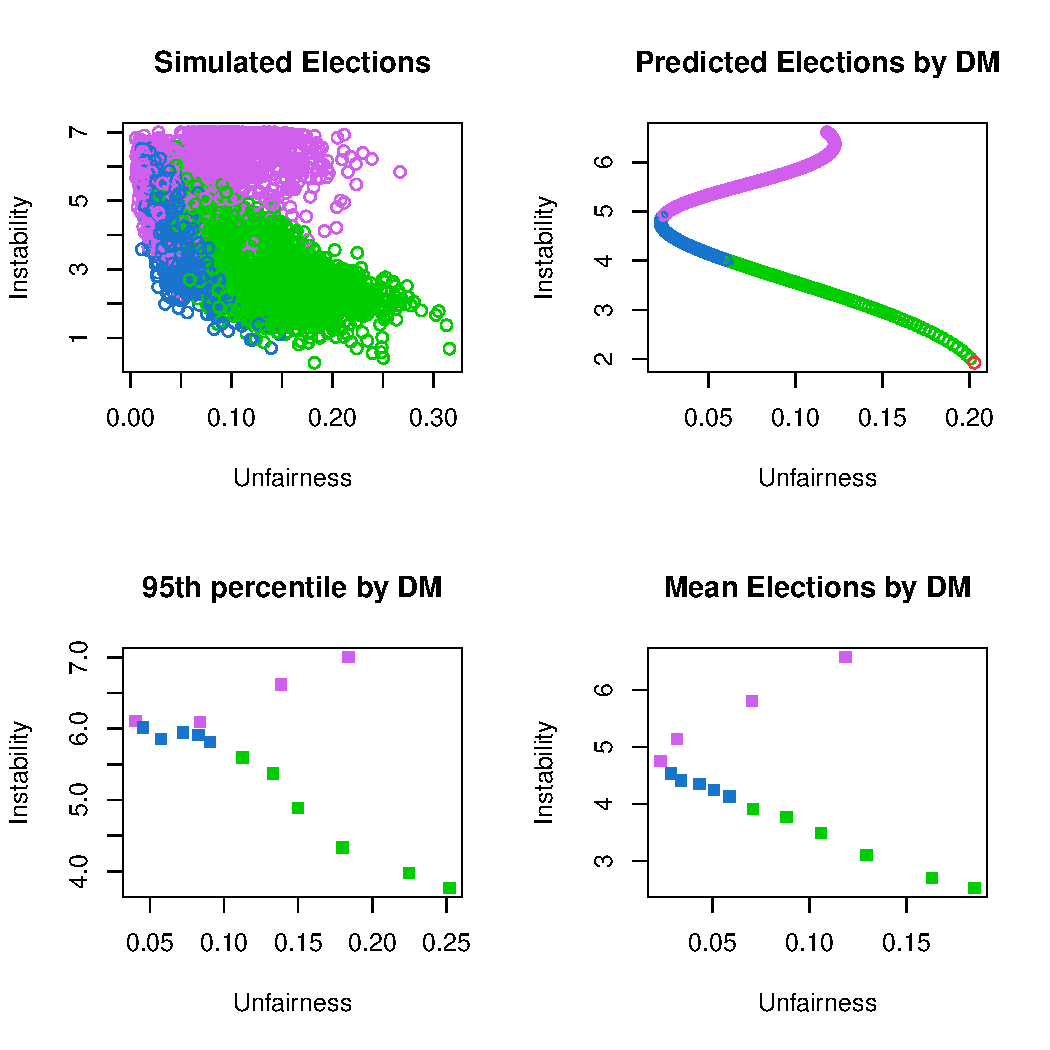
\includegraphics[scale=1.00]{images/stv_spatial2pure_gallagher_enp.pdf}
\caption{Results from simulated elections with the \emph{Spatial Model} with \emph{$2$ dimensions} and the \emph{STV} rule. Does not include major left and right parties. Plotted using the \emph{Gallagher} Index vs. \emph{ENP}. DM=1 (Red) DM=2-9 (Green) DM=10-29 (Blue) DM$>$30 (Purple)}
\label{fig:stv_spatial2pure}
\end{figure}

\begin{figure}[]
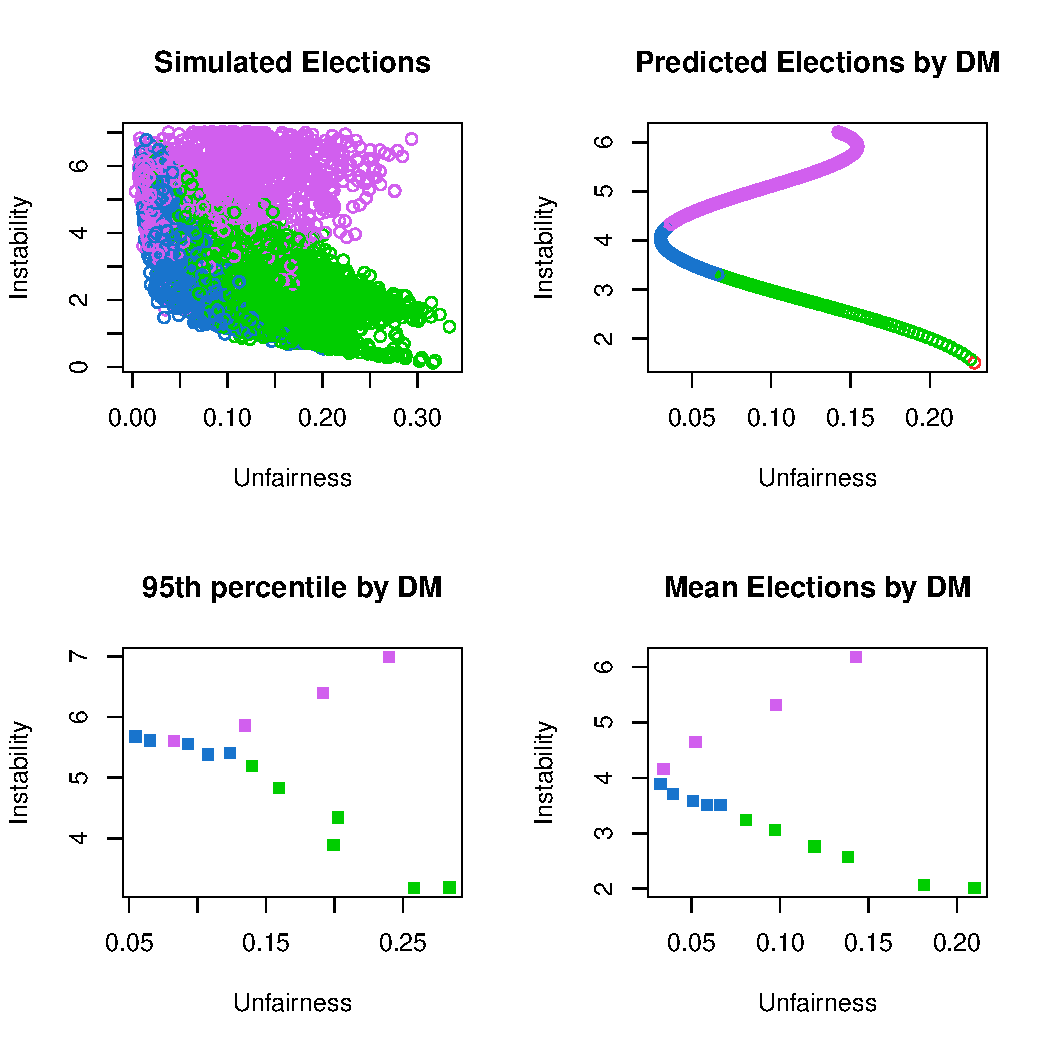
\includegraphics[scale=1.00]{images/stv_spatial1_gallagher_enp.pdf}
\caption{Results from simulated elections with the \emph{Spatial Model} with \emph{$1$ dimension} and the \emph{STV} rule. Plotted using the \emph{Gallagher} Index vs. \emph{ENP}. DM=1 (Red) DM=2-9 (Green) DM=10-29 (Blue) DM$>$30 (Purple)}
\label{fig:stv_spatial1}
\end{figure}

\begin{figure}[]
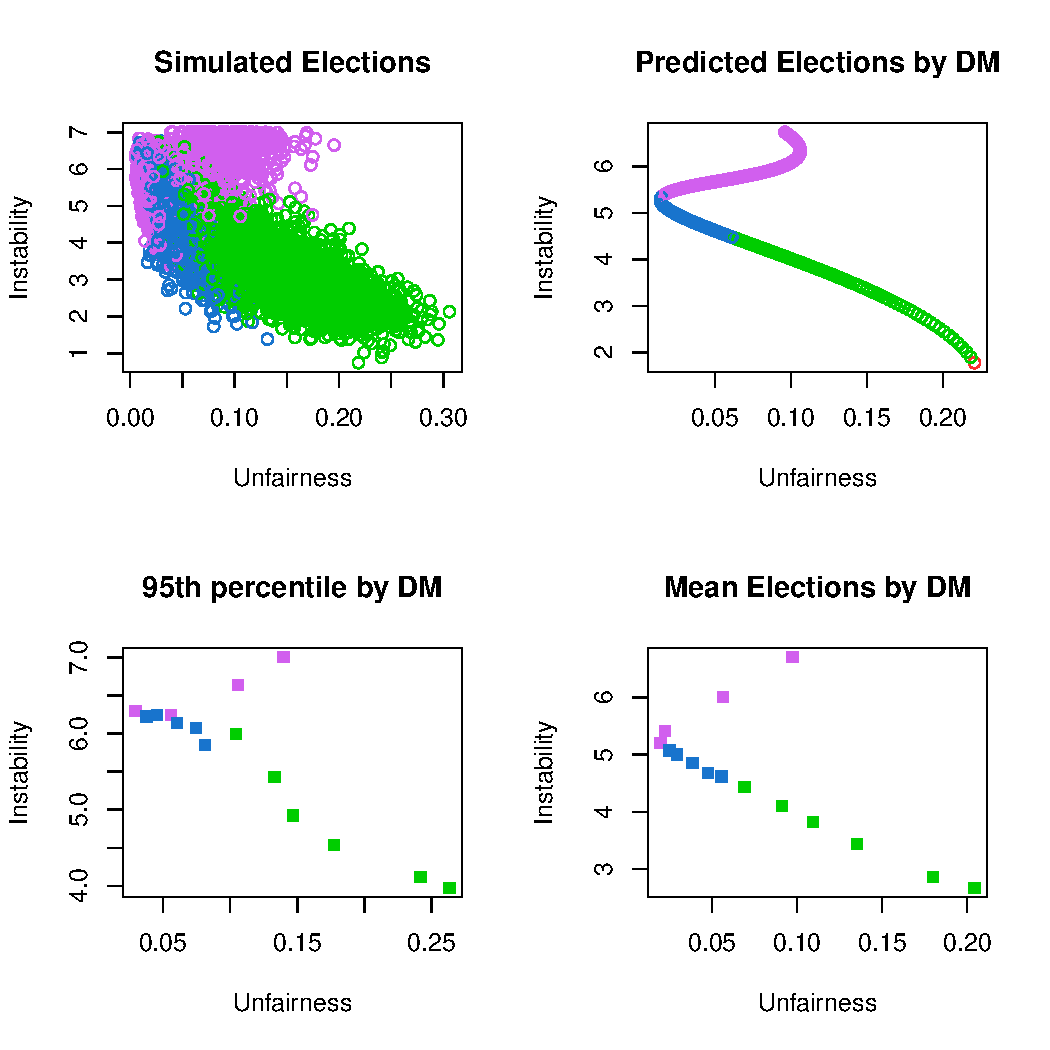
\includegraphics[scale=1.00]{images/stv_spatial3_gallagher_enp.pdf}
\caption{Results from simulated elections with the \emph{Spatial Model} with \emph{$3$ dimensions} and the \emph{STV} rule. Plotted using the \emph{Gallagher} Index vs. \emph{ENP}. DM=1 (Red) DM=2-9 (Green) DM=10-29 (Blue) DM$>$30 (Purple)}
\label{fig:stv_spatial3}
\end{figure}

\begin{figure}[]
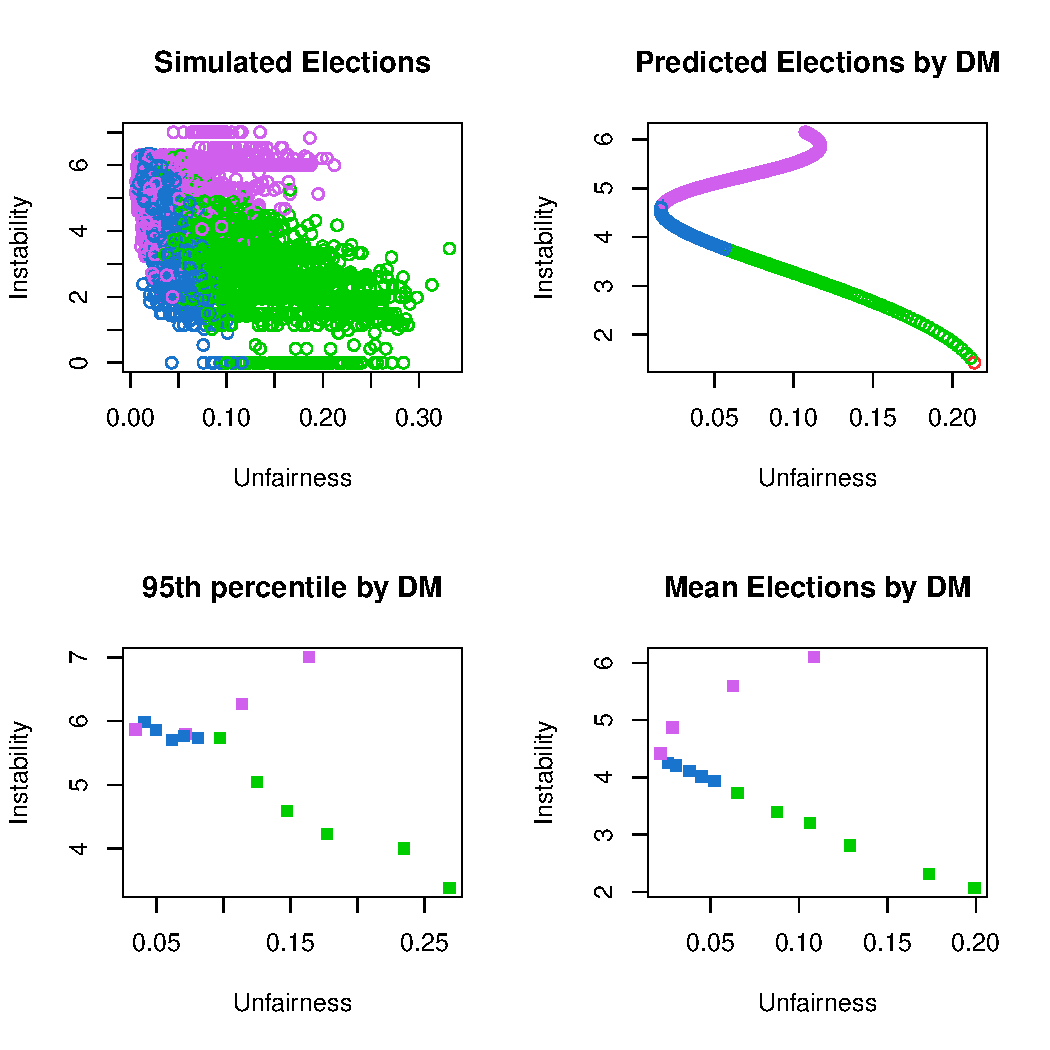
\includegraphics[scale=1.00]{images/stv_spatial2_gallagher_enpsspi.pdf}
\caption{Results from simulated elections with the \emph{Spatial Model} with \emph{$2$ dimensions} and the \emph{STV} rule. Plotted using the \emph{Gallagher} Index vs. \emph{ENP using SSPI}. DM=1 (Red) DM=2-9 (Green) DM=10-29 (Blue) DM$>$30 (Purple)}
\label{fig:stv_spatial2_sspi}
\end{figure}

\begin{figure}[]
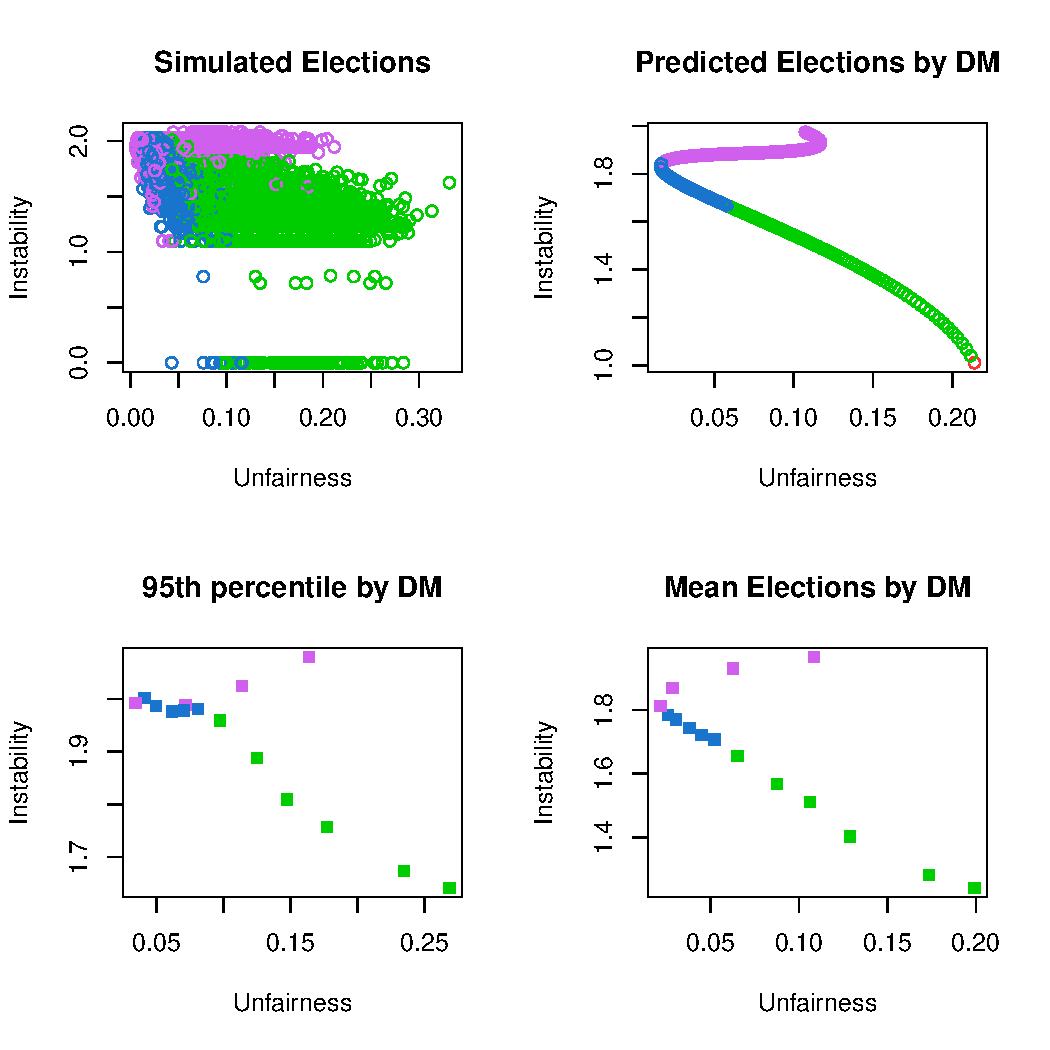
\includegraphics[scale=1.00]{images/stv_spatial2_gallagher_entropysspi.pdf}
\caption{Results from simulated elections with the \emph{Spatial Model} with \emph{$2$ dimensions} and the \emph{STV} rule. Plotted using the \emph{Gallagher} Index vs. \emph{Entropy of SSPI}. DM=1 (Red) DM=2-9 (Green) DM=10-29 (Blue) DM$>$30 (Purple)}
\label{fig:stv_spatial2_entropysspi}
\end{figure}

\begin{figure}[]
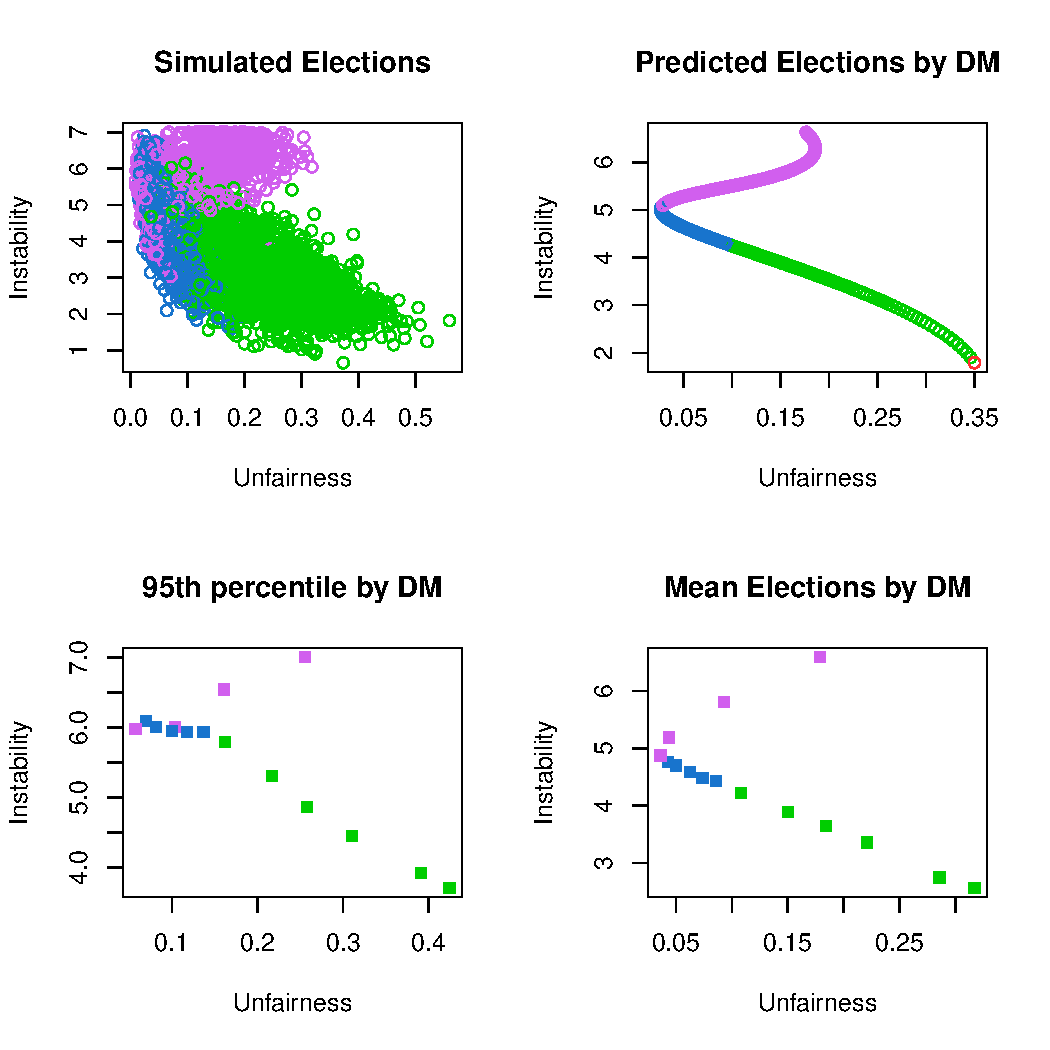
\includegraphics[scale=1.00]{images/stv_spatial2_loosemorehanby_enp.pdf}
\caption{Results from simulated elections with the \emph{Spatial Model} with \emph{$2$ dimensions} and the \emph{STV} rule. Plotted using the \emph{Loosemorehanby} Index vs. \emph{ENP}. DM=1 (Red) DM=2-9 (Green) DM=10-29 (Blue) DM$>$30 (Purple)}
\label{fig:stv_spatial2_loosemorehanby}
\end{figure}

\begin{figure}[]
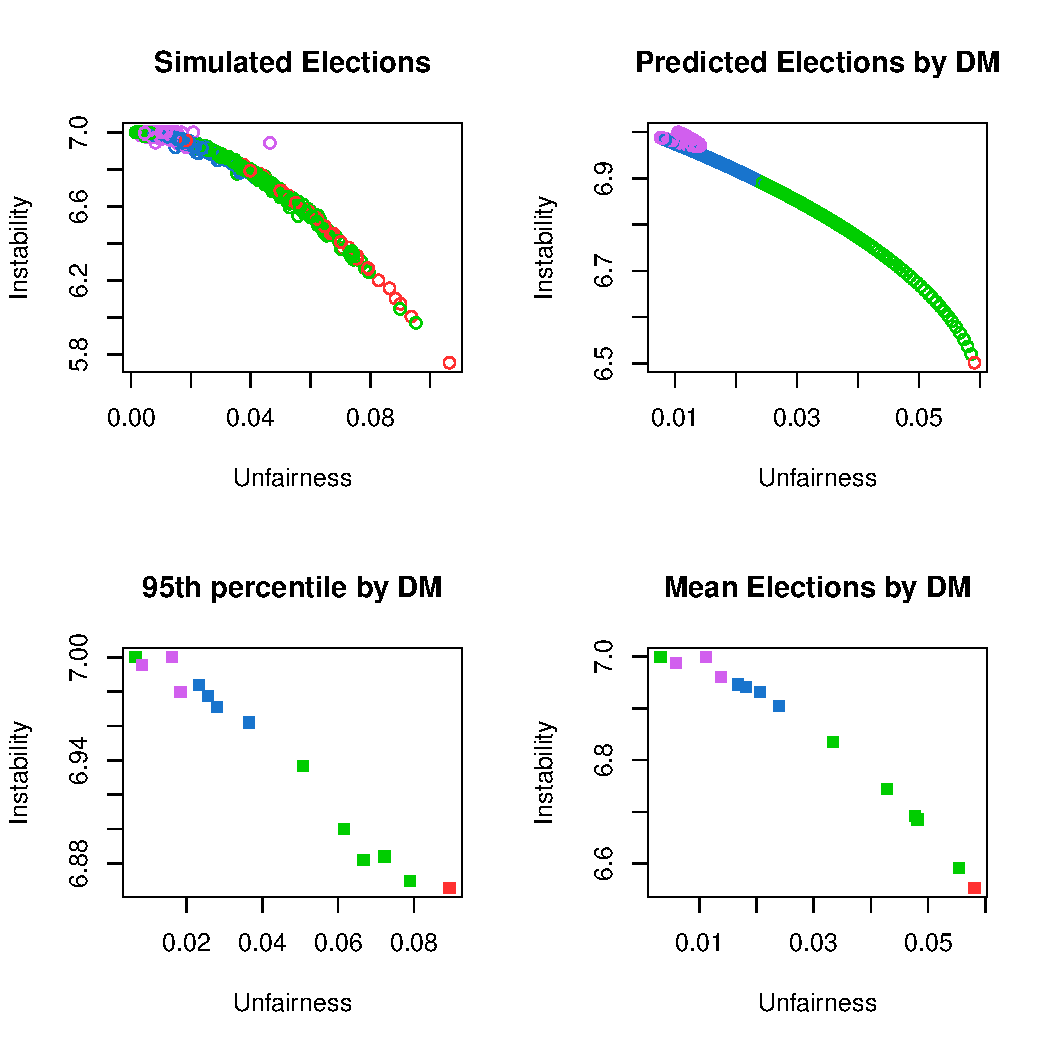
\includegraphics[scale=1.00]{images/stv_urn_gallagher_enp.pdf}
\caption{Results from simulated elections with the \emph{Polya Eggenberger Model} and the \emph{STV} rule. Plotted using the \emph{Gallagher} Index vs. \emph{ENP}. DM=1 (Red) DM=2-9 (Green) DM=10-29 (Blue) DM$>$30 (Purple)}
\label{fig:stv_urn}
\end{figure}

\begin{figure}[]
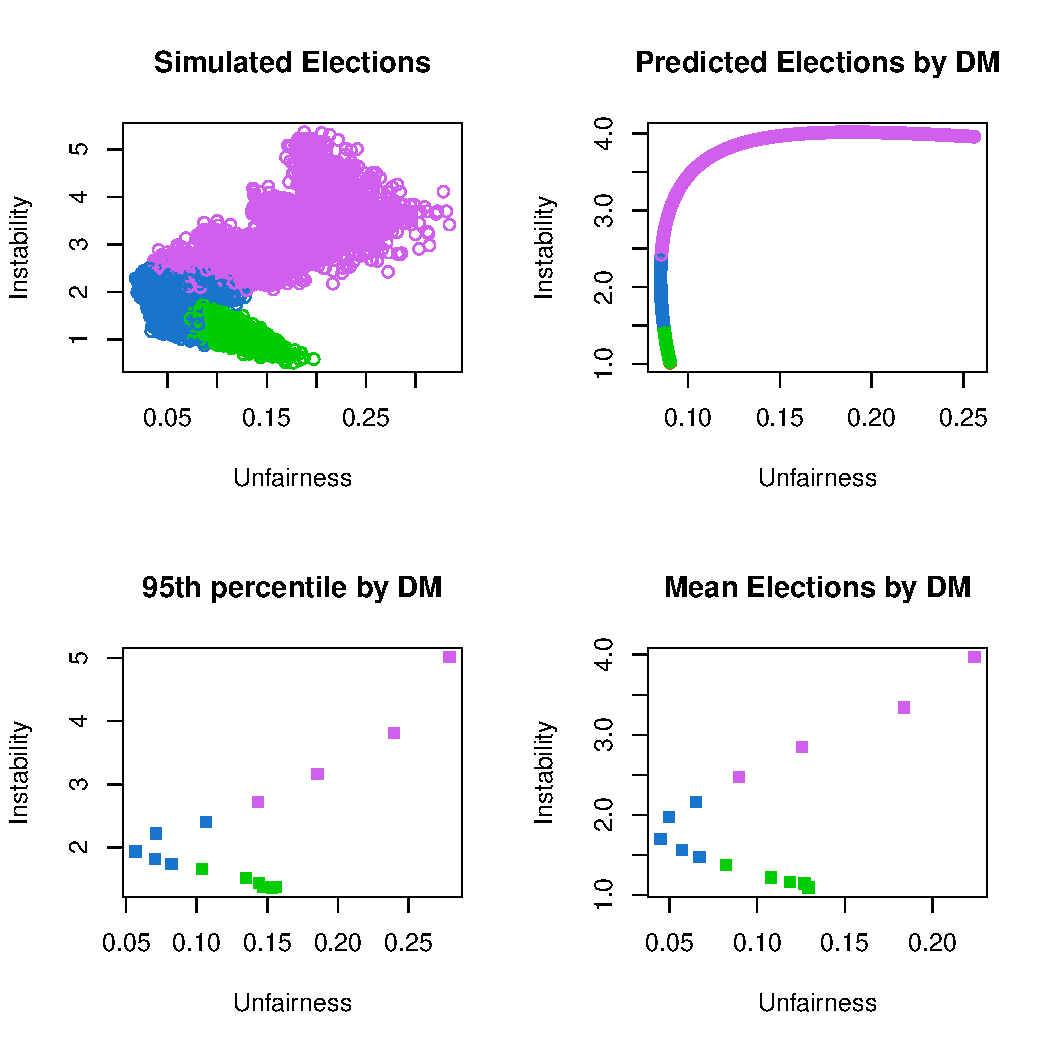
\includegraphics[scale=1.00]{images/nzprefswap_gallagher_enp.pdf}
\caption{Results from simulated elections with the \emph{Preference Swapping Model} using information from New Zealand and the \emph{STV} rule. Plotted using the \emph{Gallagher} Index vs. \emph{ENP}. DM=1 (Red) DM=2-9 (Green) DM=10-29 (Blue) DM$>$30 (Purple)}
\label{fig:stv_nzprefswap}
\end{figure}


\newpage
\subsection{Minimum Undesirability}
The following plots represent the probability of a given District Magnitude having the minimum undesirability (as defined in Section \ref{sec:undesirability}). This assumes a uniform distribution of all possible and reasonable linear undesirability functions on one measure of each unfairness and instability.

We consider all reasonable linear undesirability functions and then disregard results for the most extreme District Magnitudes, so that we do not have to make an arbitrary decision about the cut-off for extreme undesirability functions.

\begin{figure}[]
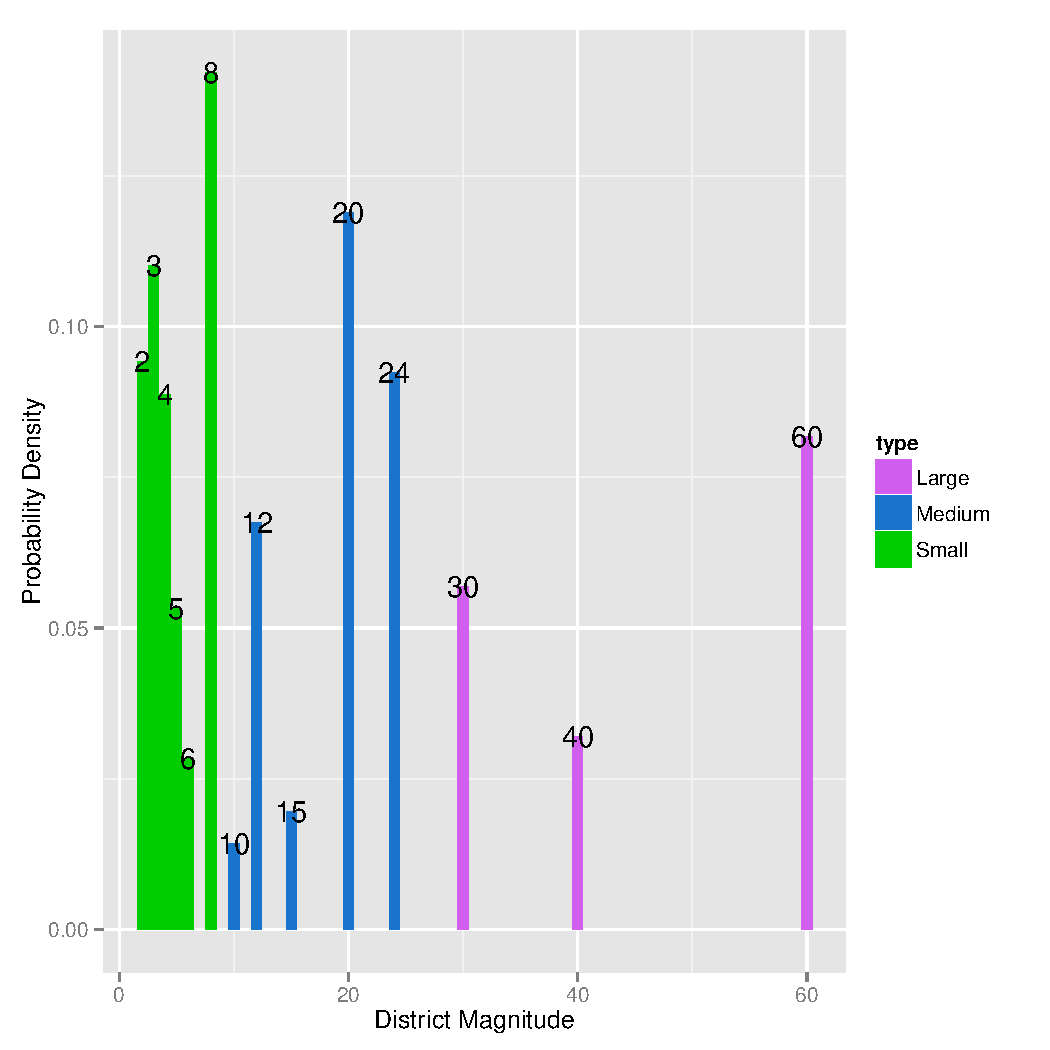
\includegraphics[scale=1.00]{images/gallagher_enp_tradeoff_overall.pdf}
\caption{Probability Distribution of least undesirable District Magnitude (including extreme values). \emph {Gallagher} and \emph{ENP}}
\label{fig:optimal_results}
\end{figure}


\begin{figure}[]
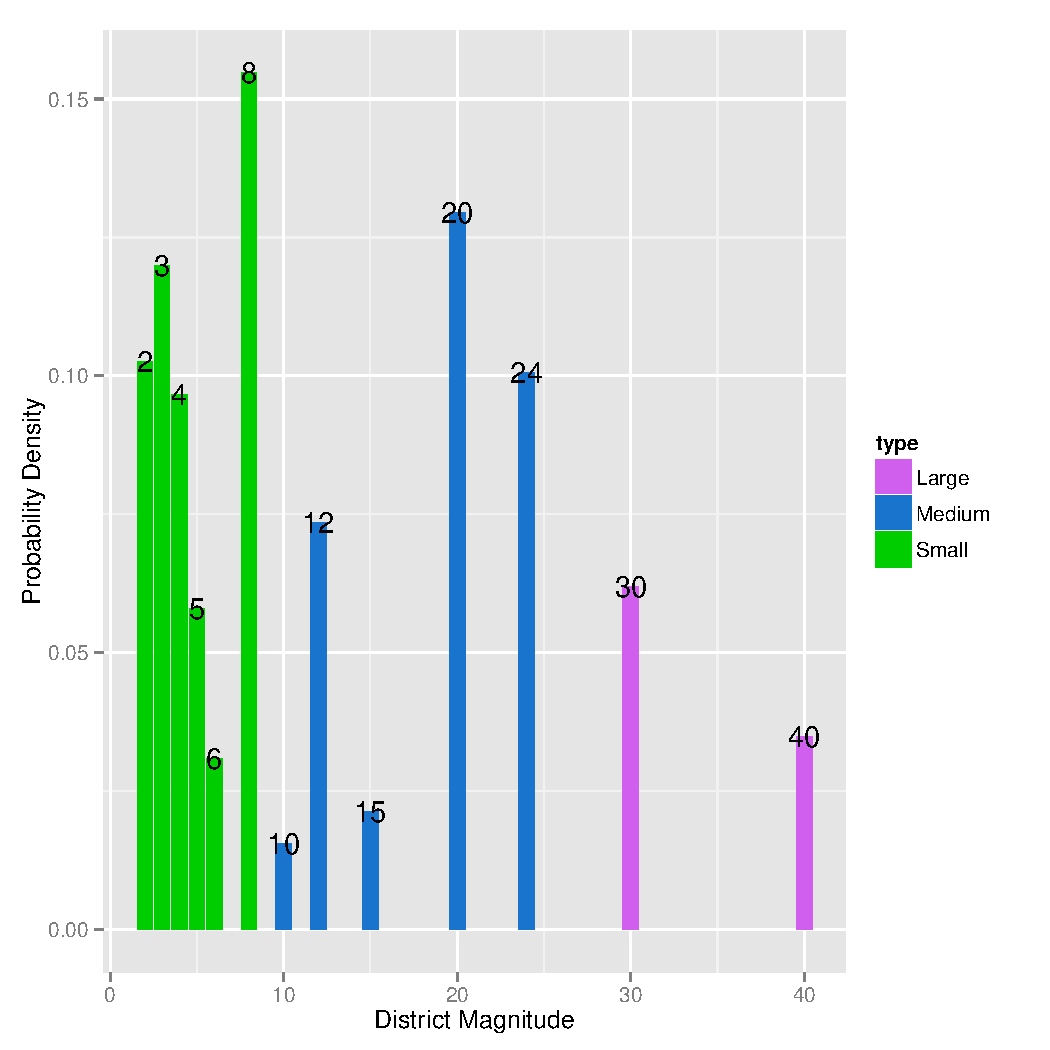
\includegraphics[scale=1.00]{images/gallagher_enp_tradeoff_overall_small.pdf}
\caption{Probability Distribution of least undesirable District Magnitude. Same results as \ref{fig:optimal_results} excluding extreme values.}
\label{fig:optimal_results_small}
\end{figure}

\begin{figure}[]
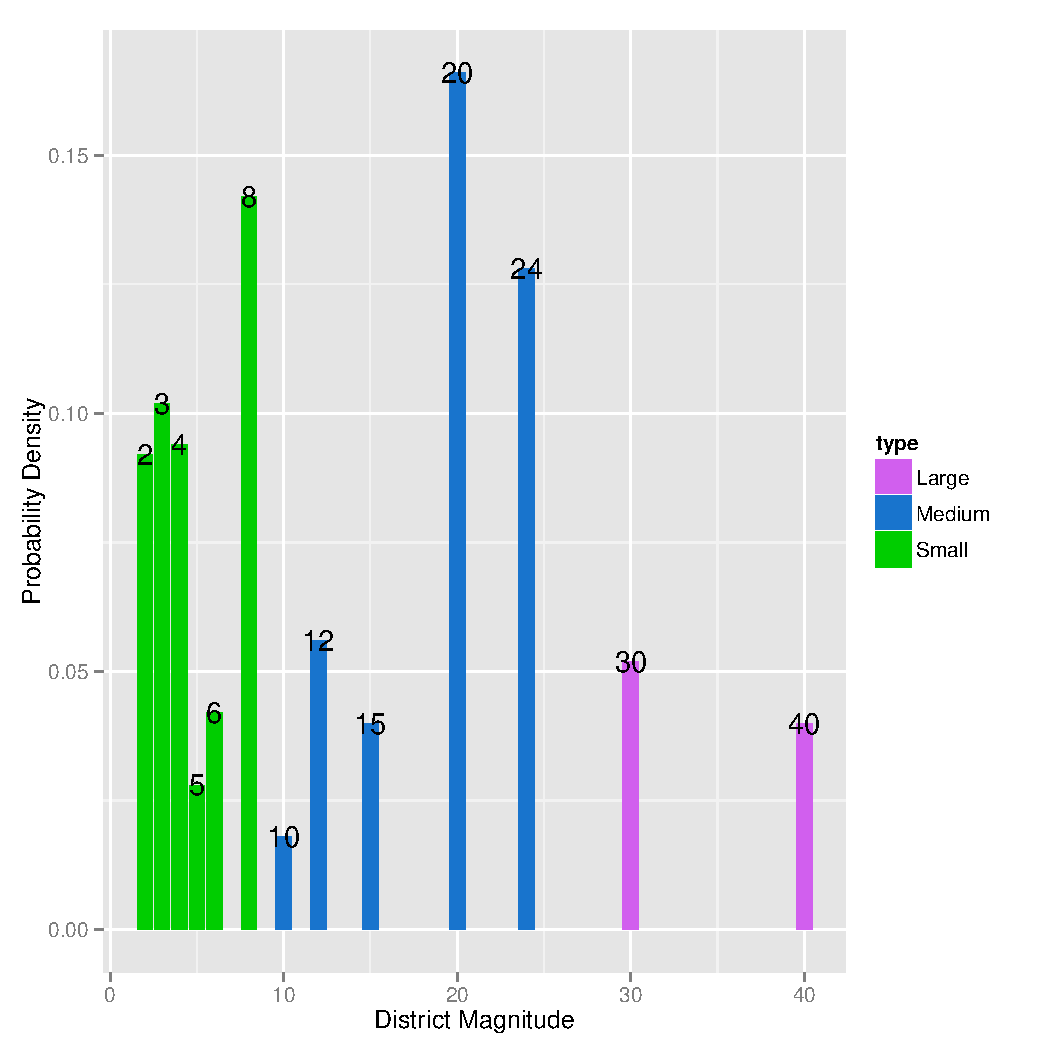
\includegraphics[scale=1.00]{images/gallagher_enpsspi_tradeoff_overall_small.pdf}
\caption{Probability Distribution of least undesirable District Magnitude. \emph {Gallagher} and \emph{ENP with SSPI}}
\label{fig:optimal_results_small_sspi}
\end{figure}

\begin{figure}[]
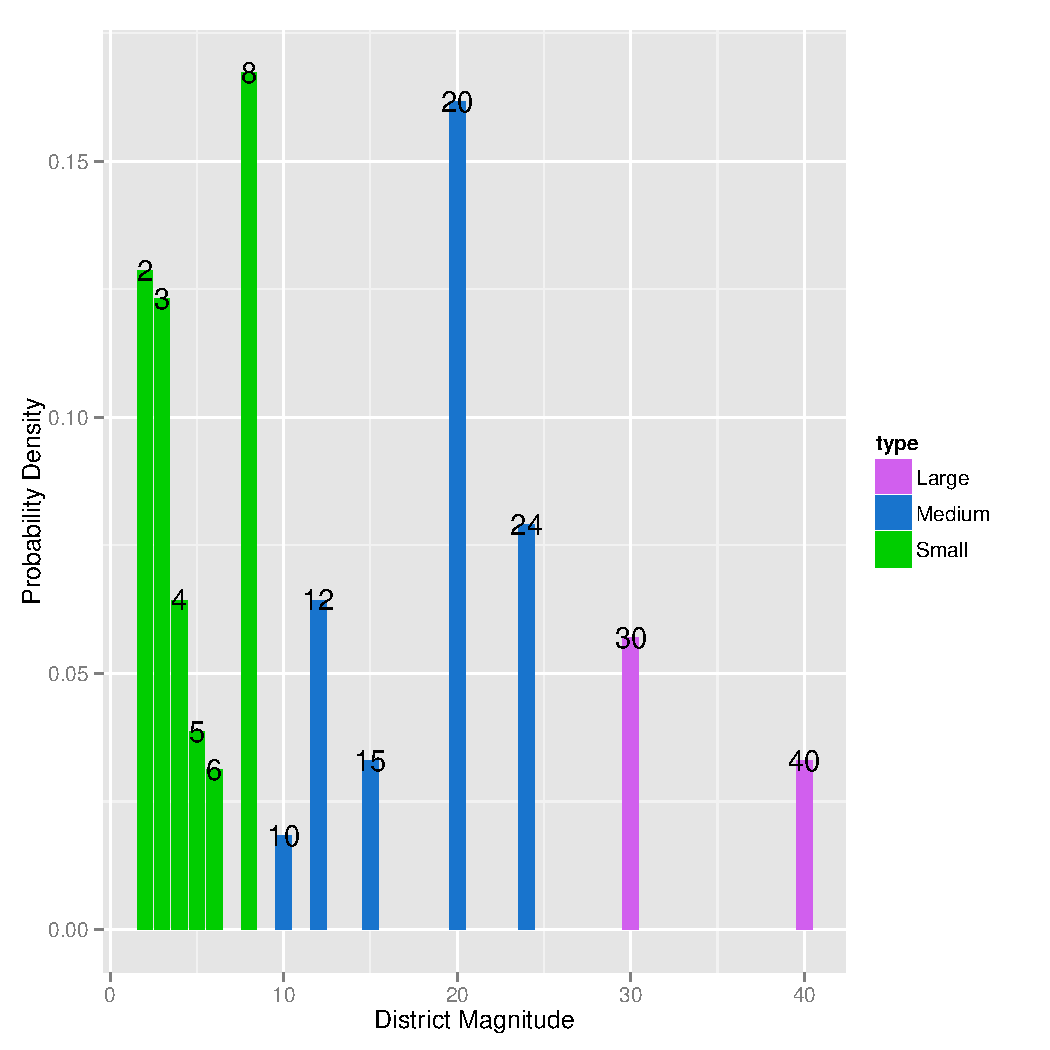
\includegraphics[scale=1.00]{images/loosemorehanby_enp_tradeoff_overall_small.pdf}
\caption{Probability Distribution of least undesirable District Magnitude. \emph {Loosemorehanby} and \emph{ENP with SSPI}}
\label{fig:optimal_results_small_loosemorehanby}
\end{figure}

\begin{figure}[]
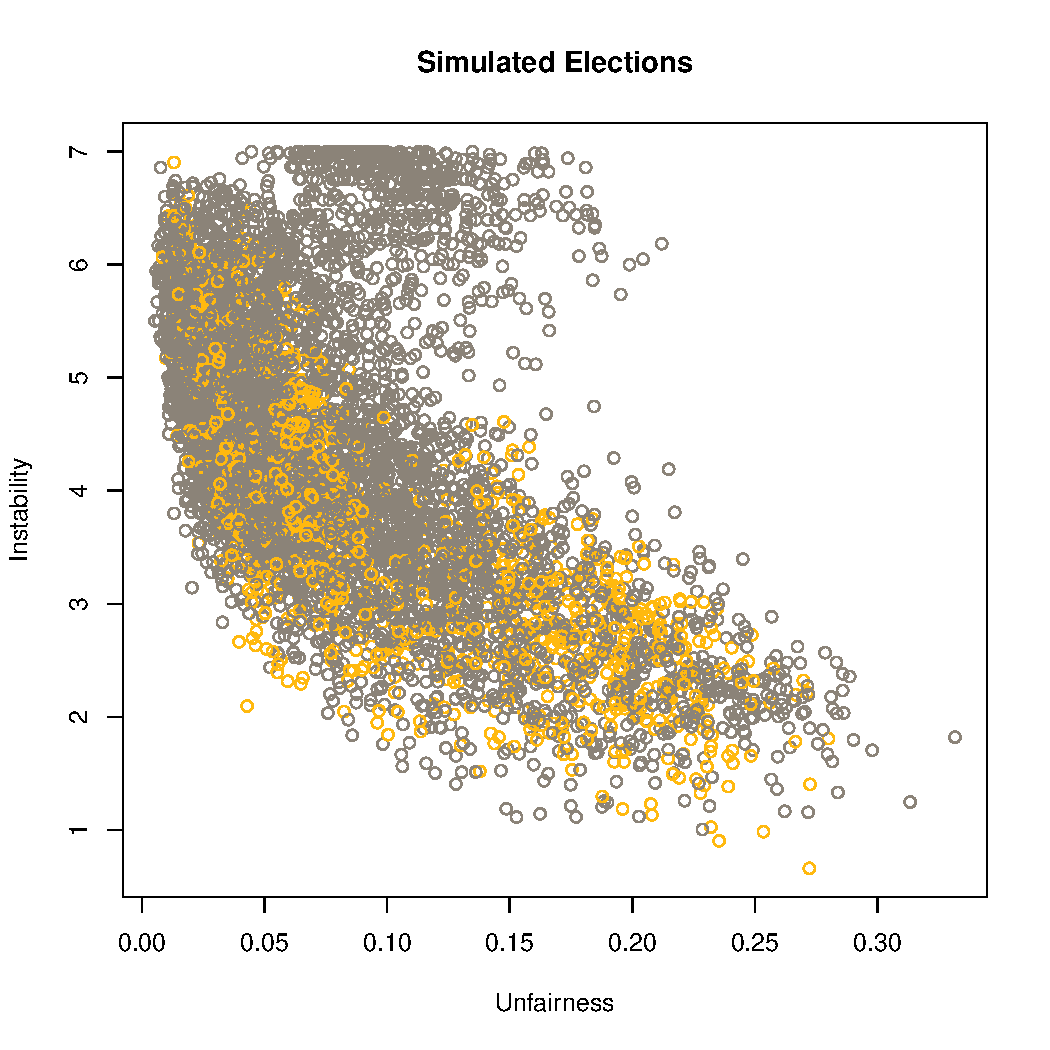
\includegraphics[scale=1.00]{images/stv_spatial2_gallagher_enp_optimal.pdf}
\caption{Results from simulated elections with the \emph{Spatial Model} with \emph{$2$ dimensions} and the \emph{STV} rule. Plotted using the \emph{Gallagher} Index vs. \emph{ENP}. "Optimal DM" (Yellow) All else (Gray)}
\label{fig:stv_spatial2_optimal}
\end{figure}

\subsection{Analysis of Different Apportionment Methods}
\label{sec:techstats}
We ran multiple simulations with the Spatial Model and the District Proportional rule, only differing by the apportionment method used in each case. We used the same District Magnitudes used in other simulation runs.

We analysed the results by creating regression fit using dummy variables for the apportionment method factors.

In the case of all our simulations, the assumption of independence between samples is satisfied by experiment design. The assumption of equal variance appears to be satisfied. 

We found extremely strong evidence of a difference in fairness \footnote{As measured by the Gallagher Index} between apportionment methods \footnote{p-value = $2.2e-16$}. We found extremely strong evidence of a difference in stability \footnote{As measured by the Effective Number of Parties} between apportionment methods \footnote{p-value = $2.2e-16$}. 

We found extremely strong evidence \footnote{p-value=0.000102} of a difference in fairness between St Lague and Hill methods. We estimate that on average fairness scores for the Hill method are between 0.35 and 1.1 percentage points higher.

We found extremely strong evidence \footnote{p-value=2e-16} of a difference in fairness between St Lague and Jefferson methods. We estimate that on average fairness scores for the Jefferson method are between 1.6 and 2.4 percentage points higher.

We found extremely strong evidence \footnote{p-value=5.51e-10} of a difference in stability between St Lague and Hill methods. We estimate that on average the ENP under the Hill method are between 0.33 and 0.17 lower.

We found extremely strong evidence \footnote{p-value=2e-16} of a difference in stability between St Lague and Jefferson methods. We estimate that on average the ENP under the Jefferson method are between 0.62 and 0.46 lower.

\newpage
\section{Discussion}
As can be seen from the plots, we found curvature in our results, however the shape of the curvature varies between models and between voting systems.

Of particular interest is the shape of the curvature in Figure \ref{fig:stv_spatial2} for very high district magnitude.

Although fairness tends to increase at the expense of stability with an increase in District Magnitude, we found that extremely high values of District Magnitude under STV have consistently worse results than for lower values of District Magnitude. In our simulations this applies to $DM>30$. This applies to the Spatial Model, preference swapping model and the Polya Eggenberger Model. There is a possibility that this effect is due to problems with our choice of measure of unfairness, in particular that the measures of unfairness used take into account only first preferences.

This effect still applies when we increase the number of districts to the much higher level of $600$. See Figure (\ref{fig:stv_spatial2large}).

Interestingly, with the District Proportional rule, we found almost the opposite effect. Likewise increasing District Magnitude tends to trade-off an increase in fairness for a decrease in stability, but extremely high values of District Magnitude tends to have higher stability than for slightly lower values of District Magnitude while still having gains in fairness.

We find that the choice of measurements has a non trivial effect on our results. For example in Figure \ref{fig:stv_spatial2}, it is debatable whether Green (DM 2-10) or Blue (DM$>$10) is optimal; as around $DM=4-6$ the trade-off is very close to linear but, at the extremes, clearly the Blue values $DM=10-29$ is optimal in the case that we favour fairness over stability and very small values $DM=2-3$ is optimal if we favour stability over fairness.

By plotting the same simulation using ENP of the Shapley Shubik Power Index (see Section \ref{sec:enppower}), Figure \ref{fig:stv_spatial2_sspi}, we find an even stronger effect than we observed on each side of $DM=4-6$. In particular $DM=3$ seems to do very well and $DM=10$ has much better 95th percentile performance than $DM=8$, in both fairness and stability.

The Loosemorehanby Index doesn't seem to have much of an effect on our results. (See Figure \ref{fig:stv_spatial2} vs. Figure \ref{fig:stv_spatial2_loosemorehanby})

The results from the preference swapping model and STV are very similar to those from the Spatial Model and STV, in contrast to the Polya Eggenberger Model and STV. This is not surprising as we would expect the preference swapping model and Spatial Model to be the most realistic and so have similar results as opposed to the highly unrealistic Polya Eggenberger.

%Undesirability.

In Figure \ref{fig:optimal_results} it is clear that the extreme values are at $DM = 1$ and $DM \geq 60$, both of which we ignore in further plots.

When plotting using the Loosemorehanby Index, we get better results for $DM=2$ than $DM=4$, however, with the Gallagher Index, $DM=3$ does much better than $DM=2$ ($DM=3$ also does well under the Gallagher Index).

There are relatively constant peaks at $DM=8$ and $DM=20$ across the different plots.

There are small values in $DM=12$ and $DM=24$. They are by comparison to other large values, much smaller, in particular when considering how close $DM=10-12$ is to the nearby peak at $DM=8$; so we ignore these.

Overall, $DM=3$, $DM=8$ and $DM=20$ seem to be the best. See Figure \ref{fig:stv_spatial2_optimal} for a comparison runs of these optimal District Magnitudes vs. non-optimal District Magnitudes.

%TODO Test with other number of seats. How does this cutoff change?

%SM
Supplementary Member has a much different curve than for the other systems. This system does very poorly in terms of both fairness and stability compared to other systems. It seems that medium to high district magnitudes around $DM=30$ are the best parameter values under this system.

%Regression fits.
The regression fits were poor due to the large amount of variation within a single class and due to the distribution of District Magnitudes we used. Unfortunately we are not able to, for example, use equally sized District Magnitudes of size $80$ in an election with $120$ seats. The regression fits showed strange behaviour around these values. We only used the regression fits for illustrative purposes so this will not have an effect on our conclusion.

%Apportionment methods.

We found that Hamilton and St Lague apportionment methods are comparable in both fairness and stability.

We found that Hill and Jefferson methods tend to trade-off fairness for stability, more so with the Jefferson method.

\newpage
\section{Conclusion}

We found extremely strong evidence of non-linearity in the results but this non-linearity mostly applies to extreme values of District Magnitude. Clearly a District Magnitude of $1$ (Red) tends to do very poorly. Performance of extremely high values compared to slightly lower values of District Magnitude varies from system to system and model to model. It appears that the trade-off in the context of small to medium sized District Magnitudes $DM=2-7$ is roughly linear.

We agree with \cite{sweetspot} that low magnitude systems tend to do better if we value each property equally, however slightly increasing or decreasing District Magnitude from this range has great effects.

We found the same general results applied when raising the number to an extremely high level.

We estimate that depending on how much fairness and stability are valued with respect to each other, optimal District Magnitude is $DM=3$, $DM=8$ or $DM=20$. We find that Supplementary Member has poor performance, however optimal DM of the largest district under SM is around $30$.

We found extremely strong evidence of a difference between the apportionment systems. We found a difference between the St Lague method and Jefferson method and a larger difference between the St Lague method and the Hill method. We found no difference between St Lague and Hamilton.

The Hill and Jefferson methods trade-off fairness for stability \footnote{When compared to St Lague}. The Jefferson method does this more so. The Jefferson method seems to gain less stability for the increase in fairness that the Hill method gets.

\section{Possible Further Research}

The artificial societies generated in these simulations assumed independent districts, which does not accurately represent the real world. It is not clear how to generate districts that are not independent.

The Spatial Model could be expanded to include more parameters. For example each voter could have an extra vector which represents how important each issue is to the voter. Distances between the voter and a given party along a given axis would then be multiplied by the corresponding value in this vector to calculate the new distance along the axis.

All of the measures of unfairness used only take into account the first preferences of voters. It is not clear how to measure unfairness by taking into account complete preference orders. This may be the cause of extreme values of District Magnitude under STV having poor results for fairness under our simulations.

This simulation assumes all voters vote sincerely. In reality this assumption is simply not true due for example to tactical voting. It is possible that certain voting systems or parameters for these voting systems have different susceptibility to tactical voting. In order to accommodate this, we would need some method of transforming true preference orders to modified tactical preference orders. It may be possible to approximate this process iteratively. For example, we could loop some large number of times, with each iteration we would select a number of like voters and check whether switching their tactical vote results in these voters getting better representation. Voters that get better representation in this case would keep this new tactical vote with some probability. It is unclear how we would measure whether or not a particular voter gets better representation, in particular taking into account their full preference orders.

%TODO More references
\clearpage
\bibliographystyle{apalike}
\bibliography{CS380Refs}

\newpage
\appendix
\section{FSharp Sourcecode}

%TODO: Clearance for this code? Can we actually use it? Do we need to cite?
% Thanks to http://www.latex-community.org/forum/viewtopic.php?f=44&t=6681&start=0 for the FSharp formatting
\definecolor{bluekeywords}{rgb}{0.13,0.13,1}
\definecolor{greencomments}{rgb}{0,0.5,0}
\definecolor{turqusnumbers}{rgb}{0.17,0.57,0.70}
\definecolor{redstrings}{rgb}{0.5,0,0}

\lstdefinelanguage{FSharp}
{morekeywords={let, new, match, with, rec, open, module, namespace, type, of, member, and, for, in, do, begin, end, fun, function, try, mutable, if, then, else, seq, yield},
keywordstyle=\color{bluekeywords},
sensitive=false,
morecomment=[l][\color{greencomments}]{///},
morecomment=[l][\color{greencomments}]{//},
morecomment=[s][\color{greencomments}]{{(*}{*)}},
morestring=[b]",
breaklines=true,  %My edit
stringstyle=\color{redstrings}
}
% End copied formatting

%TODO: Put FSharp code here.
\lstinputlisting[language=FSharp]{"C:/Users/Michael/Documents/Visual Studio 11/Projects/CS380/HypothesisTesting/Program2.fs"}

\newpage
\section{R Sourcecode}

%TODO: Any other R code? Which R code do we want to actually include.
\lstinputlisting[language=R,breaklines=true]{"C:/Users/Michael/Documents/Visual Studio 11/Projects/CS380/R/nzspatial.r"}
\lstinputlisting[language=R,breaklines=true]{"C:/Users/Michael/Documents/Visual Studio 11/Projects/CS380/R/analysis.r"}
\lstinputlisting[language=R,breaklines=true]{"C:/Users/Michael/Documents/Visual Studio 11/Projects/CS380/HypothesisTesting/bin/Debug/apportionment/analysis2.r"}

\end{document}



